% !TEX root =main.tex


%\section{Sub Protocols}




\section{Definition of Multi-party PSI with Fair Compensation and Reward}


In this section, we upgrade \p to ``multi-party PSI with Fair Compensation and Reward'' (\ep), which (in addition to offering the features of \p) allows honest clients who contribute their set to receive a reward by a buyer who initiates the PSI computation and is interested in the result.


%In this section, we present the notion of ``Earn while You Reveal PSI'' (\ep), which allows honest clients who contribute their set to get paid by a buyer who initiates the PSI computation and is interested in the result. 

%In this section, we present an efficient  PSI that allows honest parties who contribute their set to get paid by a buyer who initiates the PSI computation and is interested in the result. 

%\subsection{The Model}

%In this section, we provide the security model of our smart-PSI protocol. There are two kind of parties involved in the protocol. Namely, (1) a set of clients $\{A_{\st 1},...,A_{\st m}\}$ potentially \emph{rational} (i.e. an adversary that picks the best strategy to maximise its profit) and all may collude with each other, and (2) a non- colluding dealer: client $D$, potentially semi-honest (i.e. a passive adversary).  Similar to F-PSI, we consider static adversary, we assume there is an authenticated private (off-chain) channel between the clients and we consider a standard public blockchain.
%  


In \ep, there are (1) a set of clients $\{A_{\st 1},...,A_{\st m}\}$ a subset of which is potentially active adversaries and may collude with each other, (2) a non-colluding dealer, $D$, potentially semi-honest, and (3) an auditor $Aud$ potentially semi-honest, where all clients (except \aud) have input set. Furthermore,  in \ep  there are two ``extractor'' clients, say $A_{\st 1}$ and $A_{\st 2}$, where $(A_{\st 1},A_{\st 2})\in \{A_{\st 1},...,A_{\st m}\}$. These extractor clients volunteer to extract the (encoded) elements of the intersection and send them to a public bulletin board, i.e., a smart contract. In return, they will be paid. 
%
%We assume these two extractors are corrupted by an active adversary during interacting with other parties (and clients) until they collaborate with the rest of the clients to compute the intersection; 
%
We assume these two extractors act rationally only when they want to carry out the paid task of extracting the intersection and reporting it to the smart contract, so they can maximise their profit.\footnote{Thus, similar to any $A_{\st i}$ in \p, these extractors might be corrupted by an active adversary during the PSI computation.} For simplicity, we let client $A_{\st m}$ be the buyer, i.e., the party which initiates the PSI computation and is interested in the result. 


 The formal definition of \ep is built upon the definition of \p (presented in Section \ref{sec::F-PSI-model}); nevertheless, in \ep, we ensure that honest non-buyer clients receive a \emph{reward} for participating in the protocol and revealing a portion of their inputs deduced from the result. We:  (i)  upgrade the predicate \qdel to  \qdelwr to ensure that when honest clients receive the result, then an honest non-buyer client receives its deposit back plus a reward and a buyer client receives its deposit back minus the paid reward, and (ii) upgrade the predicate  \qUnFAbt to \qUnFAbtwr to ensure when an adversary aborts in an unfair manner (i.e., aborts but learns the result) then an honest party receives its deposit back plus a predefined amount of compensation plus a reward.  The other two predicates (i.e., \qinit and \qFAbt) remain unchanged. Given the above changes, we denote the four predicates as $\bar Q:=(\qinit,  \qdelwr, \qUnFAbtwr, \qFAbt)$. Below, we present the formal definition of predicates \qdelwr and \qUnFAbtwr. 
 
 
 

    \begin{definition}  [\qdelwr:
    %
    Delivery-with-Reward predicate] Let $\mathcal{G}$ be a stable ledger, $adr_{\st sc}$ be smart contract $sc$'s address, $adr_{\st i}\in Adr$ be the address of an honest party, $\xc$ be a fixed amount of coins, and $pram:=(\mathcal{G}, adr_{\st sc}, \xc)$. Let $R$ be a reward function that takes as input the computation result: $res$, a party's address: $adr_{\st i}$, a reward a party should receive for each unit of revealed information:  $\lc$, and input size: $inSize$.  Then $R$ is defined as follows, if $adr_{\st i}$ belongs to a non-buyer, then it returns the total amount that $adr_{\st i}$ should be rewarded and if $adr_{\st i}$ belongs to a buyer client, then it returns the reward's leftover that the buyer can collect, i.e., $R(res, adr_{\st i}, \lc, inSize)\rightarrow \rewci$.    Then, the delivery with reward predicate $\qdelwr(pram,  adr_{\st i}, res, \lc, inSize)$ returns $1$ if $adr_{\st i}$ has sent $\xc$ amount to $sc$ and received at least $\xc+\rewci$ amount from it. Else, it returns $0$. 
    
    
    
    %
%    Let also $G$ be a compensation function that takes as input  two parameters $(deps, m')$, where $deps$ is the amount of coins  that all $m+1$ parties  deposit; it returns the amount of compensation each honest party must receive, i.e., $G(deps, m')\rightarrow c'$. 
    %

 %
  \end{definition}





   \begin{definition}  [\qUnFAbtwr: UnFair-Abort-with-Reward predicate]
   %
 Let $pram:=(\mathcal{G}, adr_{\st sc}, \xc)$ be the parameters defined above, and $Adr'\subset Adr$ be a set containing honest parties' addresses, $m' = |Adr'|$,  and   $adr_{\st i}\in Adr'$. Let also $G$ be a compensation function that takes as input  three parameters $(\depsc, adr_{\st i}, m')$, where $\depsc$ is the amount of coins that all $m+1$ parties deposit, $adr_{\st i}$ is an honest party's address, and $m' = |Adr'|$; it returns the amount of compensation each honest party must receive, i.e., $G(\depsc, ard_{\st i}, m')\rightarrow \xci$. Let $R$ be the reward function defined above, i.e., $R(res, adr_{\st i}, \lc, inSize)\rightarrow \rewci$, and let $\hat {pram}:=(res, \lc, inSize)$.  Then, predicate \qUnFAbtwr is defined as $\qUnFAbtwr(pram, \hat {pram}, G, R, \depsc, m', adr_{\st i})\rightarrow (a,b)$, where $a=1$ if $adr_{\st i}$ is an honest party's address which has sent $\xc$ amount to $sc$ and received  $\xc+\xci+\rewci$  from it, and $b=1$ if $adr_{\st i}$ is an auditor's address which received $\xci$  from $sc$. Otherwise, $a=b=0$. 
  %
  \end{definition}

 
Next, we present the formal definition of multi-party PSI with Fair Compensation and Reward, \ep. 


%%%%%%%%


\begin{definition}[\ep]\label{def::PSI-Q-fair-reward}
Let $f^{\st \text{PSI}}$ be the multi-party PSI functionality defined in Section \ref{sec::F-PSI-model}. We say  protocol $\Gamma$ realises  $f^{\st \text{PSI}}$ with $\bar Q$-fairness-and-reward in the presence of $m-3$ static active-adversary clients $A_{\st j}$s and $two$ rational clients $A_{\st i}s$ or a static passive dealer  $D$ or passive auditor $Aud$, if for every non-uniform probabilistic polynomial time adversary $\mathcal{A}$ for the real model, there exists a non-uniform probabilistic polynomial-time adversary (or simulator) $\mathsf{Sim}$ for the ideal model, such that for every $I\in \{A_{\st 1},...,A_{\st m}, D, Aud\}$, it holds that: 
%
\begin{equation*}
\{\mathsf {Ideal}^{\st \mathcal{W}(f^{\st \text{PSI}}, \bar Q)}_{\st \mathsf{Sim}(z), I}(S_{\st 1},..., S_{\st m+1})\}_{\st S_{\st 1},..., S_{\st m+1},z}\stackrel{c}{\equiv} \{\mathsf{Real}_{\st \mathcal{A}(z), I}^{\st \Gamma}(S_{\st 1},..., S_{\st m+1}) \}_{\st S_{\st 1},..., S_{\st m+1},z}
\end{equation*}
where  $z$ is an auxiliary input given to $\mathcal{A}$ and  $\mathcal{W}(f^{\st \text{PSI}}, \bar Q)$ is a functionality that wraps $f^{\st \text{PSI}}$ with predicates $\bar Q:=(\qinit,  \qdelwr, \qUnFAbtwr, \qFAbt)$. 
  \end{definition}



%%%%%%%%


\section{\withRew: A Concrete Construction of \ep}


\subsection{Main Challenges to Overcome}

\subsubsection{Rewarding Clients Proportionate to the Intersection Cardinality.}
In PSIs, the main private information about the clients which is revealed to a result recipient is the private set elements that the clients have in common. Thus, honest clients must receive a reward proportionate to the intersection cardinality, from a buyer. To receive the reward, the clients need to reach a consensus on the intersection cardinality. The naive way to do that is to let every client find the intersection and declare it to the smart contract. Under the assumption that the majority of clients are honest, then the smart contract can reward the honest result recipient (from the buyer's deposit). Nevertheless, the honest majority assumption is strong in the context of multi-party PSI. Moreover, this approach requires all clients to extract the intersection, which would increase the overall costs.  Some clients may not even be interested in or available to do so. This task could also be conducted by a single entity, such as the dealer; but this approach would introduce a single point of failure and all clients have to depend on this entity.  
%
To address these challenges, we allow any two clients to become extractors.  Each of them finds and sends to the contract the (encrypted) elements in the intersection. It is paid by the contract if the contract concludes that it is honest. This allows us to avoid (i) the honest majority assumption, (ii) requiring all clients to find the intersection, and (iii) relying on a single trusted/semi-honest party to complete the task. 



\subsubsection{Dealing with Extractors' Collusion.}
%
Using two extractors itself introduces another challenge; namely, they may collude with each other (and with the buyer) to provide a consistent but incorrect result, e.g., both may declare that only $s_{\st 1}$ is in the intersection while 
 the actual intersection contains $100$ set elements, including $s_{\st 1}$.  This behaviour will not be detected by a verifier unless the verifier always conducts the delegated task itself too, which would defeat the purpose of delegation. To efficiently address this issue, we use the counter-collusion smart contracts (outlined in Section \ref{Counter-Collusion-Smart-Contracts}) which creates distrust between the two extractors and incentivises them to act honestly. 

%\subsubsection{Preserving the Intersection Privacy.} As stated above, the extractors are required to prove to a smart contract that they know 




\subsection{Description of \withRew (\epsi)}

%An Overview of E-PSI}

%This section presents a protocol, called E-PSI, that realises \ep. 

\subsubsection{An Overview.} To construct  \epsi, we mainly use \fpsi, deterministic encryption, ``double-layered'' commitments, the hash-based padding technique (from Section \ref{sec::poly-rep}), and the counter-collusion smart contracts. % (described in Section \ref{Counter-Collusion-Smart-Contracts}). 
%
At a high level, \epsi works as follows. First, all clients run step \ref{gen-FPSI-cont} of \fpsi to agree on a set of parameters and \fpsi's smart contract.  They deploy another smart contract, say $\SCe$. They also agree on a secret key, $mk'$. Next, the buyer places a certain deposit into $\SCe$. This deposit will be distributed among honest clients as a reward. 
%
%All clients check the buyer's deposit and proceed to the next step if they agree with the deposit amount.  
%
The extractors and $D$ deploy one of the counter-collusion smart contracts, i.e., \SCpc. These three parties deposit a certain amount on this contract.  Each honest extractor will receive a portion of $D$'s deposit for carrying out its task honestly and each dishonest extractor will lose a portion of its deposit for acting maliciously. 
%
Then, each client encrypts its set elements (under $mk'$ using deterministic encryption) and then represents the encrypted elements as a polynomial. The reason each client encrypts its set elements is to ensure that the privacy of the plaintext elements in the intersection will be preserved from the public. 



%Then, each client represents the encryption of its set elements as a polynomial. 





%
Next, the extractors commit to the encryption of their set elements and publish the commitments. 
%
All clients (including $D$) take the rest of the steps in \fpsi using their input polynomials. This results in a blinded polynomial,  whose correctness is checked by \fpsi's smart contact. 

If  \fpsi's smart contact approves the result's correctness, then all parties receive the money that they deposited in \fpsi's contract. In this case, each extractor finds the set elements in the intersection. Each extractor proves to $\SCe$ that the encryptions of the elements in the intersection are among the commitments that the extractor previously published. 
%
If $\SCe$ accepts both extractors' proofs, then it pays each client (except the buyer) a reward, where the reward is taken from the buyer's deposit. The extractors receive their deposits back and are paid for carrying out the task honestly. Nevertheless, if $\SCe$ does not accept one of the extractors' proofs (or one extractor betrays the other), then it invokes the auditor in the counter-collusion contracts to identify the misbehaving extractor.  Then, $\SCe$ pays each honest client (except the buyer) a reward, taken from the misbehaving extractor. $\SCe$ also refunds the buyer's deposit.
%

If  \fpsi's smart contact does not approve the result's correctness and \aud identified misbehaving clients, then honest clients will receive (1) their deposit back from \fpsi's contract, and (2)  compensation and reward, taken from misbehaving clients. Moreover, the buyer and extractors receive their deposit back from $\SCe$. Figure \ref{fig:parties-interactions-in-ANE} outlines the interaction between parties. 


\begin{figure}[htp]
    \centering
    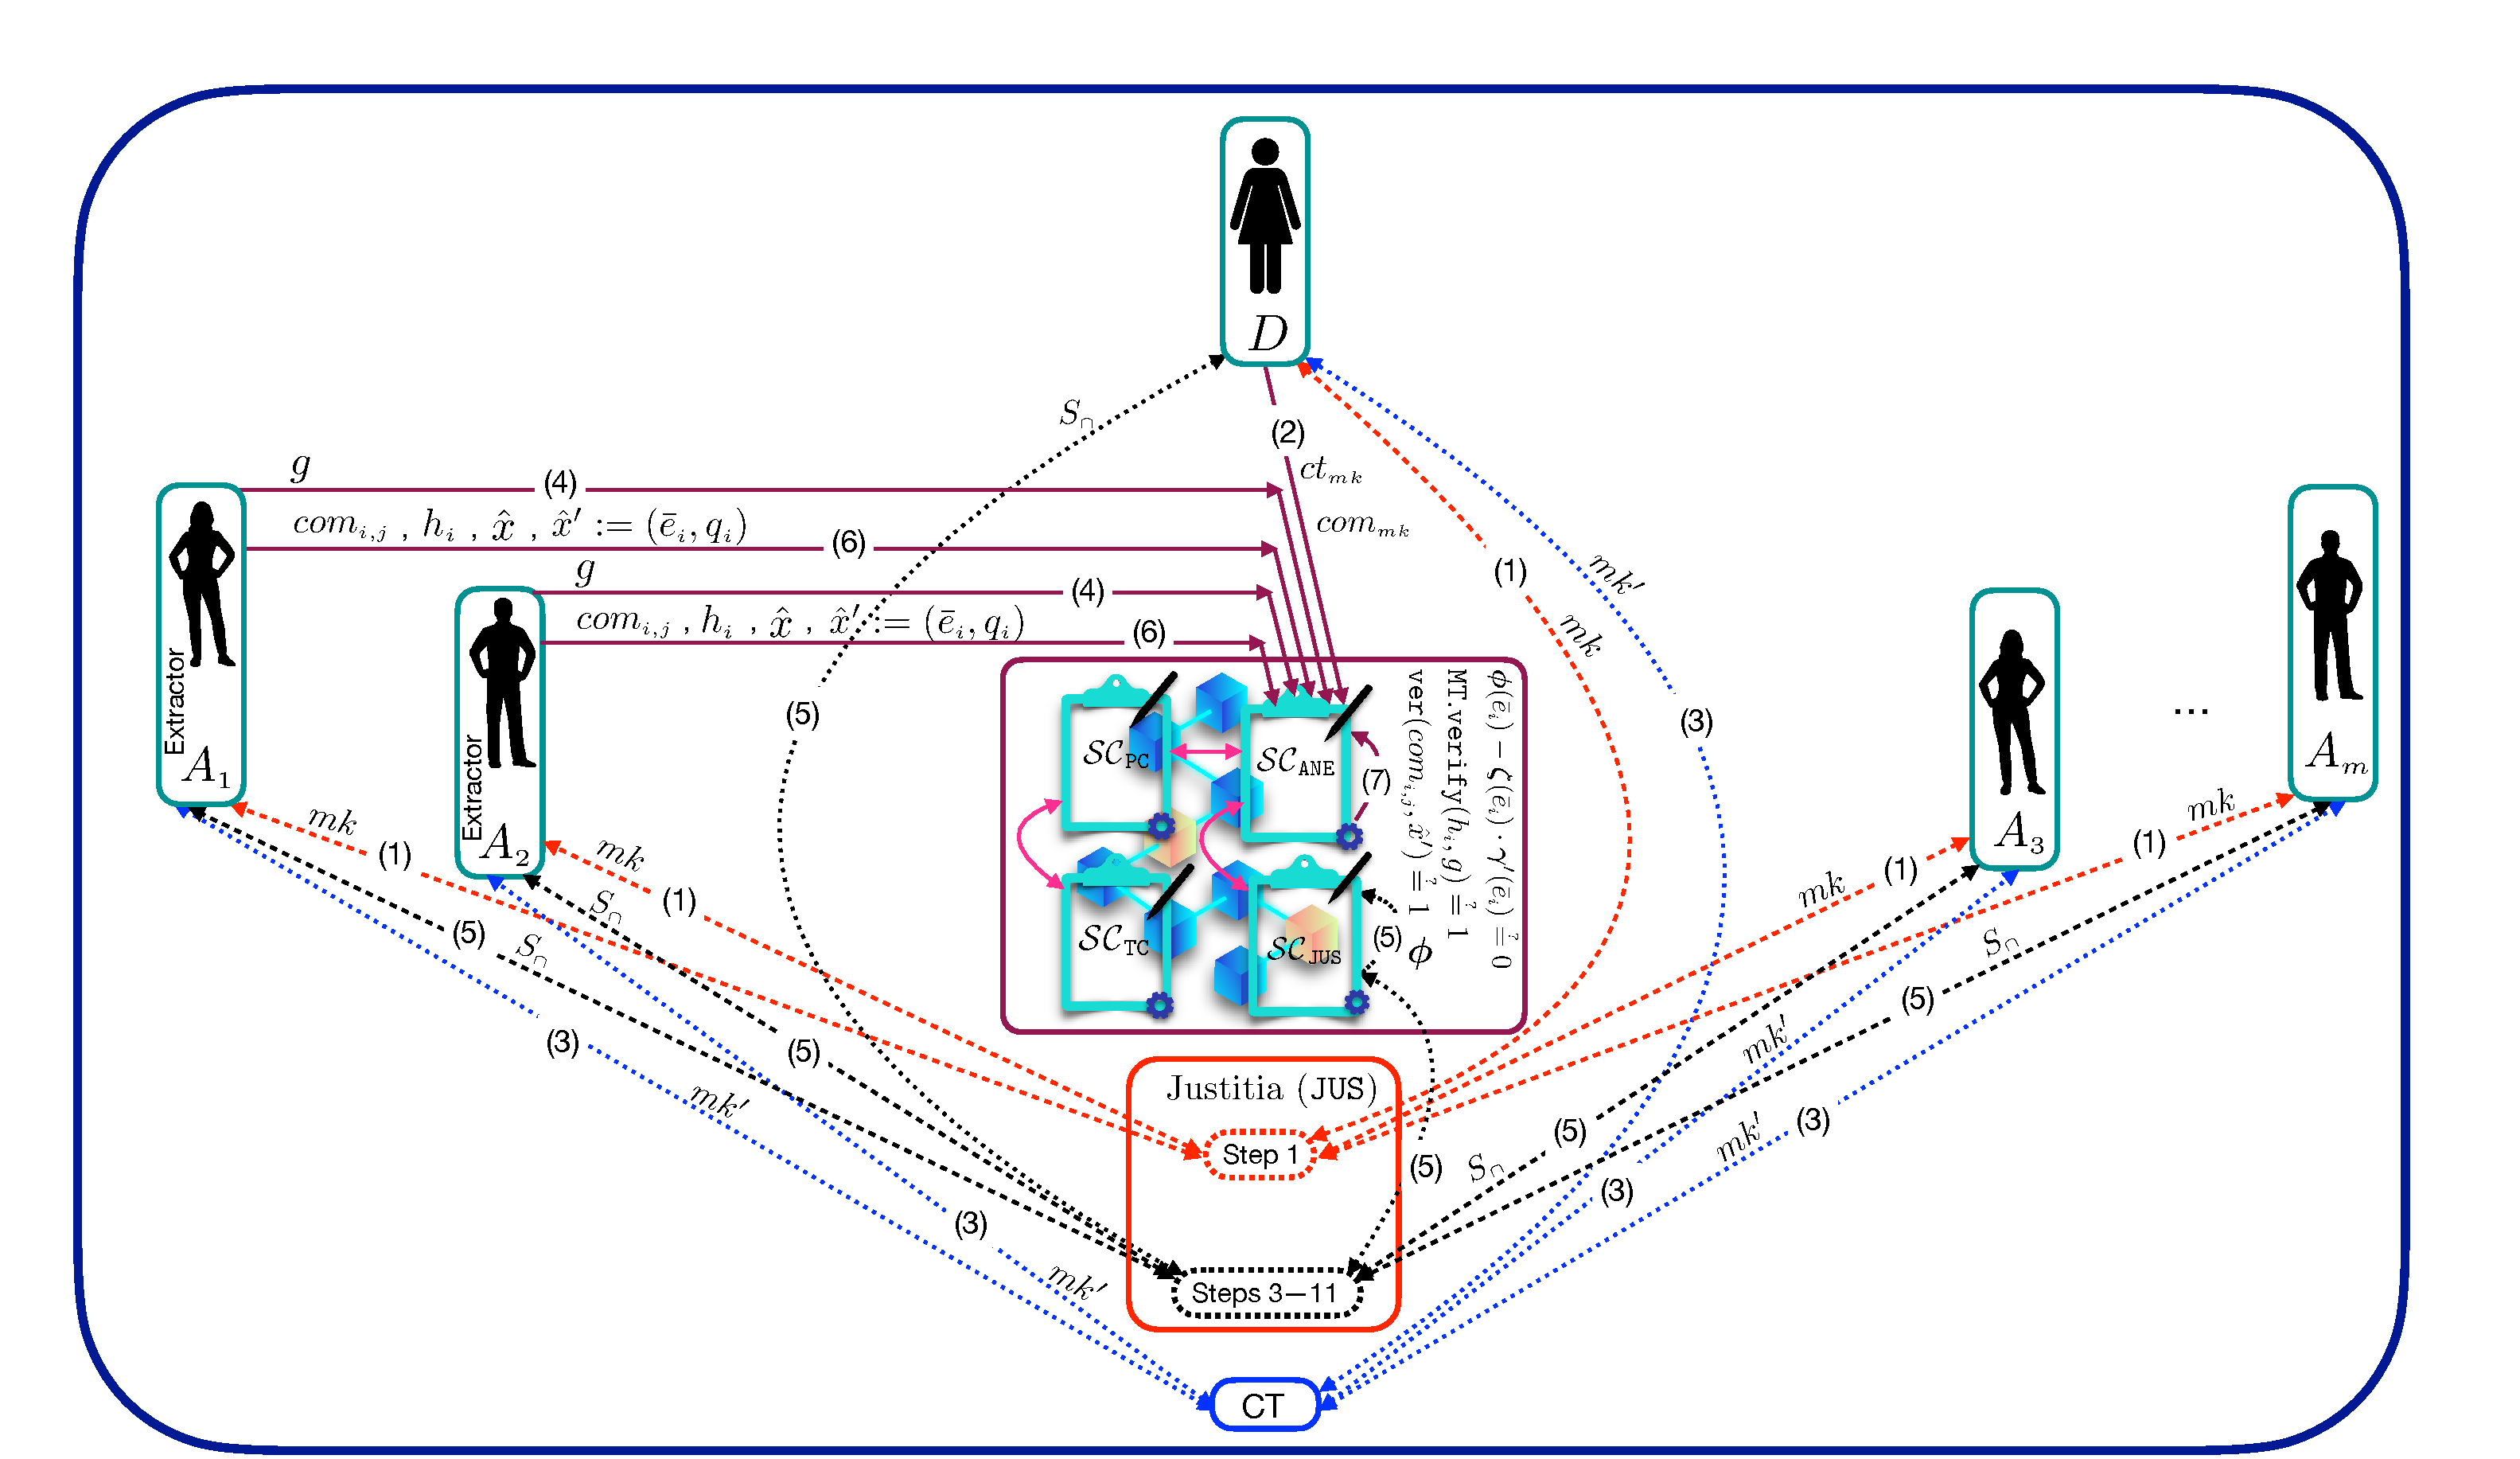
\includegraphics[width=12cm]{Diag-2.pdf}
    \caption{Outline of the interactions between parties in \withRew}\label{fig:parties-interactions-in-ANE}
\end{figure}











%However, we have to apply two essential modifications to F-PSI protocol. Generally speaking, the modifications are applied to (a) preserve the privacy of the elements in the intersection when each extractor proves the knowledge of them to the contract and (b) to identify misbehaving extractor without needing to have access to the extractor's set elements.  The role of collusion smart contracts is to create a distrust  between the extractors and buyer who may collude (out of the bound) to increase their profit.  

\subsubsection{Detailed Description of \epsi.} Next, we describe the protocol in more detail (Table \ref{table:notation-table} summarises the main notations used). 



%At a high level, two clients volunteer to be come result extractors.
%
%In the case of betray, an arbiter (potentially semi-honest) is invoked who can verify the claim of a betrayer and distribute the buyer payment among honest clients. In order for the arbiter to do so without having access to any clients input, the arbiter is required to find the intersection that requires it to find the roots of result polynomials and  be able to distinguish the error roots from actual encrypted set element. To this happen, we slightly modify the fair PSI protocol. In particular, in step \ref{encode-encrypt}, each client  $I\in \textbf{P}$ maps the elements of its set $S^{\st { {(I)}}}:\{ s^{\st { {(I)}}}_{\st 1},..., s^{\st { {(I)}}}_{\st d}\}$ to random values by encrypting them as follows. $\forall i, 1\leq i\leq d: e^{\st { {(I)}}}_{\st i}=\mathtt{PRP}(mk_{\st 2}, s^{\st { {(I)}}}_{\st i})$. Then, it encodes its encrypted set element as $ {e}^{\st { {(I)}}}_{\st i} =e^{\st { {(I)}}}_{\st i} || \mathtt{H}(e^{\st { {(I)}}}_{\st i})$.  After that, it constructs a hash table  $\mathtt{HT}^{\st { {(I)}}}$ and inserts the encrypted elements into the table. $\forall i: \mathtt{H}(  {e}_{\st i}^{\st { {(I)}}})={ {  {indx}}}$, then $  {e}^{\st { {(I)}}}_{\st i}\rightarrow \mathtt{HT}^{\st { {(I)}}}_{\st {  {indx}}}$. It pads every bin with random elements to $d$ elements (if needed). Then,  for every bin, it constructs a polynomial whose roots are  the bin's content: $\pi^{\st { {(I)}}}=\prod\limits^{\st c}_{\st i=1} (x-e'_{\st i})$, where $e'_{\st i}$ is either $ {e}^{\st {  {(I)} }}_{\st i}$, or a dummy value. 





\begin{enumerate}

%\item All clients in $\textbf{P}$ sign a smart contract $\mathcal{SC}$ and deploy it to a blockchain. Then, the buyer, $ { A}_{\st {  m}}$, deposits $v$ amounts in the contract.

\item\label{e-psi::call-F-PSI-stepOne}  All clients in $\cl=\{ A_{\st 1},...,   A_{\st m},  D\}$ together run step \ref{gen-FPSI-cont} of \fpsi (in Section \ref{Fair-PSI-Protocol}) to deploy \fpsi's contract $\mathcal{SC}_{\fpsi}$ and agree on a  master key, $mk$. 

\item\label{e-psi::deploy-SC-E-PSI} All clients in $\cl$  deploy a new smart contract, $\SCe$. The address of $\SCe$ is given to all clients. 

\item The buyer, client $ { A}_{\st {  m}}$, before time $t_{\st 1}$ deposits $\Smin\cdot \vc$  amount to $\SCe$. 
\item\label{e-PSI::buyer-deposit} All clients after  time $t_{\st 2}>t_{\st 1}$ ensure that the buyer has deposited $\Smin\cdot \vc$ amount on $\SCe$. Otherwise, they abort.



\item\label{e-PSI::extractor-deposit} $D$ signs \SCpc with the extractors. $\SCe$ transfers $\Smin\cdot \rc$ amount (from the buyer deposit) to \SCpc for each extractor. This is the maximum amount to be paid to an honest extractor for honestly declaring the elements of the intersection. %Each honest extractor will be paid $\hat w'= r\cdot |{ { {S}}}_{\st\cap}|$, where 
%
Each extractor  deposits $\dc'=\dc+\Smin\cdot \fc$ amount in \SCpc at time $t_{\st 3}$. At time $t_{\st 4}$ all clients ensure that the extractors deposited enough coins; otherwise, they withdraw their deposit and abort. 

%
\item\label{e-psi::commit-to-mk} $D$ encrypts $mk$ under the public key of the dispute resolver (in \SCpc); let $ct_{\st mk}$ be the resulting ciphertext.  It also generates a commitment of $mk$ as follows: $z'=\mathtt{PRF}(mk, 0),\ com_{\st mk}=\comcom(mk, z')$. It stores $ct_{\st mk}$  and ${com}_{\st mk}$ in $\SCe$. 


\item\label{e-psi::gen-mk-prime} All clients in $\cl$ engage in \ct to agree on another key, $mk'$.
%
\item\label{Smart-PSI:encode-elem} Each client  in $\cl$ maps the elements of its set $S:\{ s_{\st 1},..., s_{\st c}\}$ to random values by encrypting them as: $\forall i, 1\leq i\leq c: e_{\st i}=\mathtt{PRP}(mk', s_{\st i})$. 
%
Then, it encodes its encrypted set element as $\bar{e}_{\st i} =e_{\st i} || \mathtt{H}(e_{\st i})$.  
%
After that, it constructs a hash table  $\mathtt{HT}$ and inserts the encoded elements into the table. $\forall i: \mathtt{H}( \bar{e}_{\st i})={ {  {j}}}$, then $\bar{e}_{\st i}\rightarrow \mathtt{HT}_{\st {  {j}}}$. It pads every bin with random dummy elements to $d$ elements (if needed). Then,  for every bin, it builds a polynomial whose roots are the bin's content: $\bm\pi^{\st { {(I)}}}=\prod\limits^{\st d}_{\st i=1} (x-e'_{\st i})$, where $e'_{\st i}$ is either $\bar{e}_{\st i}$, or a dummy value. 




\item\label{merkel-tree-cons} Every extractor in $\{A_{\st 1}, A_{\st 2}\}$: 

\begin{enumerate}
%
%\item for each bin, derives a pseudorandom polynomial: $\gamma'_{\st {  {j}}}$, using key $mk$.
%
%\item for each bin, evaluates $\gamma'_{\st {  {j}}}$ at the encode set elements of that bin: $\gamma'_{\st {  {j,i}}}=\gamma'_{\st {  {j}}}(\bar{e}^{\st { {(I)}}}_{\st i})$.
\item\label{smart-PSI::commit-to-bin} for each $j$-th bin, commits to the bin's elements: $com_{\st{i,j}}=\comcom(e'_{\st i}, q_{\st i})$, where $q_{\st i}$ is a fresh randomness  used for the commitment and $e'_{\st i}$ is either $\bar{e}_{\st i}$, or a dummy value of the bin. %Thus, if the bin contains paddings, it  commits to the paddings too. 




%\item commits to every  encrypted element.  $\forall i, 1\leq i\leq d: \mathtt{a}^{\st { {(I)}}}_{\st i}=\mathtt{Com}(e^{\st { {(I)}}}_{\st i}, q^{\st { {(I)}}}_{\st i})$, where $q^{\st { {(I)}}}_{\st i}$ is a fresh randomness  used for the commitment.
\item  constructs a Merkel tree on top of all committed values as follows: $\mkgen(com_{\st 1,1},...,com_{\st d,h})\rightarrow g$. %Let $\mathtt{MT}^{\st g}$ be a Merkel tree with a root node $g^{\st I}$. 
\item stores the Merkel tree's root $g$ on $\SCe$.
\end{enumerate}


\item\label{e-psi::invoke-remainer-F-PSI} All clients in $\cl$   run steps \ref{ZSPA}--\ref{compute-res-poly} of \fpsi, where each client now deposits (in the $\mathcal{SC}_{\fpsi}$) $\yc'$ amount where $\yc'>\Smin\cdot \vc+{\chc}$. Recall, at the end of step \ref{compute-res-poly}  of \fpsi for each $j$-th bin (i) a random polynomial $\bm\zeta$ has been registered in $\mathcal{SC}_{\fpsi}$, (ii) a polynomial $\bm\phi$ (blinded by a random polynomial $\bm\gamma'$) has been extracted by $\mathcal{SC}_{\fpsi}$, and (iii) $\mathcal{SC}_{\fpsi}$  has checked this polynomial's  correctness. If the latter check:

\begin{itemize}
\item[$\bullet$] passes (i.e., $Flag=True$): all parties run step \ref{F-PSI::flag-is-true} of \fpsi (with a minor difference, see Section \ref{sec::Discussion-Anesidora}).  In this case, each party receives $\yc'$ amount it deposited in $\mathcal{SC}_{\fpsi}$. They proceed to step \ref{smart-PSI::extractors} below.
\item[$\bullet$]  fails (i.e., $Flag=False$): all parties run step \ref{F-PSI::flag-is-false}  of \fpsi. In this case,
(as in \fpsi) \aud is paid $\chc$ amount, and each honest party receives back its deposit, i.e., $\yc'$ amount. Also,  from the misbehaving parties' deposit  $\frac{m'\cdot \yc'-\chc}{m-m'}$ amount is sent to each honest client,  to reward and compensate the client $\Smin\cdot \lc$ and $\frac{m'\cdot \yc'-\chc}{m-m'}- \Smin\cdot \lc$ amounts respectively, where $m'$ is the total number of misbehaving parties.  Moreover, $\SCe$ returns to the buyer its deposit (i.e., $\Smin\cdot \vc$ amount paid to $\SCe$), and returns to each extractor its deposit, i.e., $\dc'$ amount paid to \SCpc. Then, the protocol halts. 
\end{itemize}

\item\label{smart-PSI::extractors} Every extractor client: 
\begin{enumerate}

\item finds the elements in the intersection. To do so, it first encodes each of its set elements to get $\bar e_{\st i}$, as explained in step \ref{Smart-PSI:encode-elem}.  
%i.e.,  it first computes $e^{\st { {(I)}}}_{\st i}=\mathtt{PRP}(mk',s^{\st { {(I)}}}_{\st i})$ and then computes $\bar{e}^{\st { {(I)}}}_{\st i} =e^{\st { {(I)}}}_{\st i} || \mathtt{H}(e^{\st { {(I)}}}_{\st i})$.
%
% and then encodes it:   (i.e. $ {e}^{\st { {(I)}}}_{\st i} =e^{\st { {(I)}}}_{\st i} || \mathtt{H}(e^{\st { {(I)}}}_{\st i})$). 
 %
 Then, it determines to which bin the encrypted value belongs, i.e., ${ {  {j}}}=\mathtt{H}( \bar{e}_{\st i})$. Next, it evaluates the resulting polynomial (for that bin) at the encrypted element. It considers the element in the intersection if the evaluation is zero, i.e., $\bm\phi( \bar{e}_{\st i})-\bm\zeta( \bar{e}_{\st i})\cdot \bm\gamma'( \bar{e}_{\st i})=0$. If the extractor is a traitor, by this point it should have signed \SCtc with $ { D}$ and provided all the inputs (e.g., correct result) to \SCtc. 

\item \label{extractor-proves} proves that every element in the intersection is among the elements it has committed to. Specifically, for each element in the intersection, say $\bar{e}_{\st i}$, it sends to $\SCe$: 



\begin{enumerate}
%
%\item [$\bullet$]  the opening of commitment $\mathtt{a}'$, i.e., pair $\ddot {x}:=(mk, z')$. This is done only once for all elements in the intersection.  
%
\item [$\bullet$]  commitment $com_{\st i,j}$ (generated in step \ref{smart-PSI::commit-to-bin}, for $\bar{e}_{\st i}$) and its  opening ${\hat x}':=(\bar{e}_{\st i},  q_{\st i})$. 


%
%\item [$\bullet$] the element's commitment: $\mathtt{a}^{\st { {(I)}}}_{\st {  {j,i}}}=\mathtt{Com}(\gamma'_{\st {  {j,i}}}, q^{\st { {(I)}}}_{\st i})$, where $q^{\st { {{(I)}}} }_{\st i}$ was generated in step \ref{merkel-tree-cons}.   
%
%\item[$\bullet$]  $ \bar{e}^{\st { {{(I)}}} }_{\st i}$ and it  commitment's opening:  $\mathtt{m}^{\st { {{(I)}}} }_{\st i}=(\gamma'_{\st {  {j,i}}}, q^{\st { {{(I)}}} }_{\st i})$. 

%
\item[$\bullet$]   proof $h_{\st i}$ that asserts $com_{\st i,j}$ is a leaf node of   a Merkel tree with  root $g$. 

%\item[$\bullet$] the index of the bin to which $ \bar{e}^{\st { {{(I)}}} }_{\st i}$ belongs, i.e., ${ {  {j}}}=\mathtt{H}(\bar {e}^{\st { {{(I)}}} }_{\st i})$. 
 \end{enumerate}
\item sends the opening of commitment $com_{\st mk}$, i.e., pair $\hat {x}:=(mk, z')$, to $\SCe$. This is done only once for all elements in the intersection.  

 \end{enumerate}
\item\label{e-psi::SC-verification} Contract $\SCe$:
%
\begin{enumerate}

\item\label{e-psi::SC-verification--derive-mk}  verifies the opening of the commitment for $mk$, i.e., $\comver(com_{\st mk},\hat{x})=1$. If the verification passes, it generates the index of the bin to which $ \bar{e}_{\st i}$ belongs, i.e., ${ {  {j}}}=\mathtt{H}(\bar {e}_{\st i})$. It  uses $mk$ to derive the pseudorandom polynomial $\bm\gamma'$ for $j$-th bin. 


 \item\label{e-psi::SC-verification--check-three-vals} checks whether (i) the opening of commitment is valid,  (ii) the Merkle tree proof is valid, and (iii) the encrypted element is the resulting polynomial's root. Specifically, it ensures that the following relation holds: 
 

$$\Bigg(\comver(com_{\st i,j}, \hat{x}')=1\Bigg) \hspace{1mm} \wedge \hspace{1mm} \Bigg(\mkver(h_{\st i},g)=1\Bigg) \hspace{1mm} \wedge \hspace{1mm}  \Bigg(\bm\phi( \bar{e}_{\st i})-\bm\zeta( \bar{e}_{\st i})\cdot \bm\gamma'( \bar{e}_{\st i})=0\Bigg)$$


%$$\mathtt{Ver_{\st com}}(\mathtt{a}^{\st { {{(I)}}} }_{\st {  {j,i}}},\mathtt{m}^{\st { {{(I)}}} }_{\st i})=1\ \ \ \ \wedge \ \ \ \ \mathtt{Ver_{\st MT}}(\mathtt{h}^{\st { {{(I)}}} }_{\st i},g^{\st { {{(I)}}} })=1 \ \ \ \ \wedge \ \ \ \  \phi( \bar{e}^{\st { {{(I)}}} }_{\st i})-\zeta( \bar{e}^{\st { {{(I)}}} }_{\st i})\cdot \gamma'_{\st {  {j,i}}}=0$$

%\item if all proofs of both extractors are valid and both extractors provide identical elements of the intersections (for each bin),  for each valid proof, it takes $m\cdot l$ coins from the buyer's deposit (in $\mathcal{SC}_{\st {  {EXT}}}$) and distributes it among all clients, except the buyer. 

\end{enumerate}

% !TEX root =main.tex




\item The parties are paid as follows. 

\begin{itemize}
%
\item[$\bullet$]  if the extractors' proofs are valid, they provided identical elements of the intersections (for each bin), and there is no traitor, then $\mathcal{SC}_{\epsi}$:
\begin{enumerate}
%
 \item takes $|S_{\st\cap}|\cdot m\cdot \lc$ amount from the buyer's deposit (in $\mathcal{SC}_{\epsi}$) and distributes it among all clients, excluding the buyer. 
 %
 \item calls \SCpc which returns the extractors' deposit (i.e., $\dc'$ amount each) and pays each extractor $|S_{\st\cap}|\cdot \rc$ amount, for doing their job correctly. 
  %
 \item checks if $|{ { {S}}}_{\scriptscriptstyle\cap}|<\Smin$. If the check passes, then it returns $(\Smin-|S_{\scriptscriptstyle\cap}|)\cdot \vc$ amount  to the buyer.
 %
 \end{enumerate}
% 
\item[$\bullet$] if both extractors failed to deliver any result, then $\mathcal{SC}_{\epsi}$:
%
\begin{enumerate}
%
\item refunds the buyer, by sending $\Smin\cdot \vc$ amount (deposited in $\mathcal{SC}_{\epsi}$) back to the buyer. 
%
\item retrieves each extractor's deposit from \SCpc and distributes it among the rest of the clients (excluding the buyer and extractors).  
%
 \end{enumerate}
 %
 \item[$\bullet$]\label{smart-PSI-inconsistency} Otherwise (e.g., if some proofs are invalid, if an extractor's result is inconsistent with the other extractor's result, or there is a traitor), $\mathcal{SC}_{\epsi}$ invokes (steps 8.c and 9 of) \SCpc and its auditor to identify the misbehaving extractor, with the help of $ct_{\st mk}$ after decrypting it. $\mathcal{SC}_{\epsi}$ asks \SCpc to pay the auditor the total amount of $\chc$ taken from the deposit of the extractor(s) who provided incorrect result to $\mathcal{SC}_{\epsi}$. Moreover,
%

\begin{enumerate}
%
\item if \underline{both extractors cheated}:
%
\begin{enumerate}[leftmargin=2mm]
%
\item\label{both-cheated-no-traitor} if there \underline{is no traitor}, then $\mathcal{SC}_{\epsi}$ refunds the buyer, by sending $\Smin\cdot \vc$ amount (deposited in $\mathcal{SC}_{\epsi}$) back to the buyer. It also distributes $2\cdot \dc'- \chc$ amount (taken from the extractors' deposit in \SCpc) among the rest of  the clients  (excluding the buyer and extractors). %The Prisoner's contract pays its dispute resolver $ch$ amount. 
%
%
\item if there \underline{is a traitor}, then:
%%%%%
\begin{enumerate}
%
%
\item\label{both-cheated-honest-traitor} if the traitor delivered a \underline{correct result} in \SCtc, $\mathcal{SC}_{\epsi}$ retrieves $\dc'-\dc$ amount from the other dishonest extractor's deposit (in \SCpc) and distributes it among the rest of the clients (excluding the buyer and dishonest extractor). It asks \SCpc to send $|S_{\st\cap}|\cdot \rc+\dc'+\dc-\chc$ amount to the traitor (via \SCtc). % and $\hat{ch}$ amount to the dispute resolver.
%
\SCtc refunds the traitor's deposit, i.e., $\chc$ amount. It refunds the buyer, by sending $\Smin\cdot \vc-|S_{\st\cap}|\cdot \rc$ amount (deposited in $\mathcal{SC}_{\epsi}$) to it.


 %Otherwise (i.e., if it delivered an incorrect result in the Traitor's contract), the Traitor's contract refunds the traitor's deposit (i.e., $ch$ amount).
%
\item if the traitor delivered an \underline{incorrect result} in \SCtc, then $\mathcal{SC}_{\epsi}$ pays the buyer and the rest of the clients in the same way it does in step \ref{both-cheated-no-traitor}. 
%
%distributes $2\cdot \hat d- \hat{ch}$ amount (taken from the extractors deposit in the Prisoner's contract) among the rest of the clients (except the buyer and extractors). 
%
%The Prisoner's contract pays its dispute resolver $\hat{ch}$ amount.
%
\SCtc refunds the traitor,  $\chc$ amount.  %It refunds the buyer, by sending ${\resizeT {\textit {S}}}_{\resizeS {\textit  min}}\cdot v$ amount (deposited in $\mathcal{SC}_{\resizeS {\textit  {EXT}}}$) back to the buyer.


%
\end{enumerate}
%%%%%
\end{enumerate}
%
\item if \underline{one of the extractors cheated}: 
%
\begin{enumerate}[leftmargin=2mm]
%
\item if there \underline{is no traitor},  $\mathcal{SC}_{\epsi}$ calls \SCpc that (a) returns the honest extractor's deposit ($\dc'$ amount), (b) pays this extractor $|S_{\st\cap}|\cdot \rc$ amount, for doing its job honestly, and (c) pays this extractor $ \dc-\chc$ amount taken from the dishonest extractor's deposit. 
%
%and (d) pays its dispute resolver $\hat {ch}$ amount taken from the dishonest extractor's deposit. 
%
%Also, $\mathcal{SC}_{\resizeS {\textit  {EXT}}}$ sends ${\resizeT {\textit {S}}}_{\resizeS {\textit  min}}\cdot v-|S_{\st\cap}|\cdot r$ amount (deposited in $\mathcal{SC}_{\resizeS {\textit  {EXT}}}$) back to the buyer.
%
 $\mathcal{SC}_{\epsi}$ pays the buyer and the rest of the clients in the same way it does in step \ref{both-cheated-honest-traitor}. 


% It retreives  $\hat d - \hat c - \hat{ch}$ amount from the dishonest extractor's deposit (in the Prisoner’s contract) and distributes it among the rest of clients (except the buyer and dishonest extractor). %
%
\item if there \underline{is a traitor}
%
%%%%%


\begin{enumerate}
%
\item\label{one-cheated-exists-traitor-honest-traitor}  if the traitor delivered a \underline{correct result} in \SCtc (but  cheated in $\mathcal{SC}_{\epsi}$),  $\mathcal{SC}_{\epsi}$ calls \SCpc that (a) returns the other honest extractor's deposit ($\dc'$ amount), (b) pays the honest extractor $|S_{\st\cap}|\cdot \rc$ amount taken from the buyer's deposit, for doing its job honestly,  (c) pays the honest extractor $\dc- \chc$ amount taken from the traitor's deposit,  
%
%(d) pays its dispute resolver $\hat{ch}$ amount taken from the traitor extractor's deposit (deposited in $\mathcal{SC}_{\resizeS {\textit  {EXT}}}$), 
%
 (d)
 pays to the traitor $|S_{\st\cap}|\cdot \rc$ amount taken from the buyer’s deposit (via the \SCtc), and (e) refunds the traitor $\dc'-\dc$ amount taken from its own deposit.  \SCtc refunds the traitor's deposit, $\chc$ amount.  $\mathcal{SC}_{\epsi}$ takes $|S_{\st\cap}|\cdot m\cdot \lc$ amount from the buyer's deposit (in $\mathcal{SC}_{\epsi}$) and distributes it among all clients, excluding the buyer. If $|{ { {S}}}_{\scriptscriptstyle\cap}|<\Smin$,   $\mathcal{SC}_{\epsi}$ returns $(\Smin-|{ { {S}}}_{\scriptscriptstyle\cap}|)\cdot \vc$ amount (from $\mathcal{SC}_{\epsi}$)  to the buyer. 
 
 
%
\item  if the traitor delivered an \underline{incorrect result} in \SCtc (and it cheated in $\mathcal{SC}_{\epsi}$), then $\mathcal{SC}_{\epsi}$ pays the honest extractor in the same manner as it did in step \ref{one-cheated-exists-traitor-honest-traitor}.  
%
%calls Prisoner's contract that (a) returns the other honest extractor's deposit (i.e., $\hat d$ amount), (b) pays the honest extractor $|S_{\st\cap}|\cdot r$ amount, for doing its job honestly, and (c) pays the honest extractor $\hat c$ amount taken from the traitor extractor's deposit. 
%
%, and  (d) pays its dispute resolver $\hat{ch}$ amount taken from the traitor extractor's deposit (deposited in $\mathcal{SC}_{\resizeS {\textit  {EXT}}}$). 
%
\SCtc refunds the traitor's deposit, i.e., $\chc$ amount. 
%
%$\mathcal{SC}_{\resizeS {\textit  {EXT}}}$ takes ${\resizeT {\textit {S}}}_{\resizeS {\textit  min}} \cdot f$ amount from the traitor's deposit (in $\mathcal{SC}_{\resizeS {\textit  {EXT}}}$) and distributes it among all clients, except the buyer and traitor. 
%
%Also, $\mathcal{SC}_{\resizeS {\textit  {EXT}}}$ sends ${\resizeT {\textit {S}}}_{\resizeS {\textit  min}}\cdot v-|S_{\st\cap}|\cdot r$ amount (deposited in $\mathcal{SC}_{\resizeS {\textit  {EXT}}}$) back to the buyer. 
%
Also, $\mathcal{SC}_{\epsi}$ pays the buyer and the rest of the clients in the same way it does in step \ref{both-cheated-honest-traitor}.


%
\end{enumerate}


\end{enumerate}

\end{enumerate}
\end{itemize}



%
%\begin{enumerate}
%
%\item fully refunds the buyer, as before.
%%
%\item calls Prisoner's contract that (a) returns the honest extractor's deposit (i.e., $\hat d$ amount), (b) pays this extractor $|S_{\st\cap}|\cdot r$ amount, for doing its job honestly,  (c) pays this extractor $\hat c$ amount taken from the dishonest extractor's deposit, and (d) pays its dispute resolver $ch$ amount taken from the dishonest extractor's deposit.
%%
%\item retrieves $\hat d-\hat c- ch$ amount from dishonest extractor's deposit (in the Prisoner's contract) and distributes it among the rest of the clients (except the buyer and dishonest extractor). 
%
%\end{enumerate}
%

 
 
 %%%%%%%%%%%. without Traitor
% \item Otherwise (e.g., if some proofs are invalid or if an extractor's result is inconsistent with the other extractor's result), $\mathcal{SC}_{\resizeS {\textit  {EXT}}}$ invokes (steps 8.c and 9 of) the Prisoner's contract to identify the misbehaving extractor. 
%%
%
%\begin{itemize}
%%
%\item[$\bullet$] if both extractors cheated, then $\mathcal{SC}_{\resizeS {\textit  {EXT}}}$:
%%
%\begin{enumerate}
%%
%\item refunds the buyer, by sending ${\resizeT {\textit {S}}}_{\resizeS {\textit  min}}\cdot v$ amount (deposited in $\mathcal{SC}_{\resizeS {\textit  {EXT}}}$) back to the buyer.
%%
%\item retrieves $\hat d-ch$ amount from each extractor's deposit (in the Prisoner's contract) and distributes it among the rest of the clients (except the buyer and extractors). The Prisoner's contract pays its dispute resolver $ch$ amount for each dishonest extractor. 
%%
%\end{enumerate}
%%
%\item[$\bullet$] if one of the extractors cheated, then $\mathcal{SC}_{\resizeS {\textit  {EXT}}}$:
%%
%\begin{enumerate}
%%
%\item fully refunds the buyer, as before.
%%
%\item calls Prisoner's contract that (a) returns the honest extractor's deposit (i.e., $\hat d$ amount), (b) pays this extractor $|S_{\st\cap}|\cdot r$ amount, for doing its job honestly,  (c) pays this extractor $\hat c$ amount taken from the dishonest extractor's deposit, and (d) pays its dispute resolver $ch$ amount taken from the dishonest extractor's deposit.
%%
%\item retrieves $\hat d-\hat c- ch$ amount from dishonest extractor's deposit (in the Prisoner's contract) and distributes it among the rest of the clients (except the buyer and dishonest extractor). 
%%
%\end{enumerate}
%%
%\end{itemize}








%\item Contract $\mathcal{SC}_{\st {  {EXT}}}$ after time $t_{\st 3}$ checks if $|{ { {S}}}_{\st\cap}|<{ { {S}}}_{\st {  min}}$. In this case, it returns $({ { {S}}}_{\st {  min}}-|{ { {S}}}_{\st\cap}|)\cdot v$ amount  to the buyer.

\end{enumerate}



 \begin{theorem}\label{theorem::E-PSI-security}
If  $\mathtt{PRP}$, $\mathtt{PRF}$, the commitment scheme, smart contracts, the Merkle tree scheme, \fpsi and the counter-collusion contracts are secure and the public key encryption is semantically secure,  then  \epsi realises  $f^{\st \text{PSI}}$ with $\bar Q$-fairness-and-reward (w.r.t. Definition \ref{def::PSI-Q-fair-reward}) in the presence of $m-3$ static active-adversary clients $A_{\st j}$s and $two$ rational clients $A_{\st i}s$ or a static passive dealer $D$ or passive auditor $Aud$, or passive public which sees the intersection cardinality.
 \end{theorem}




Before we prove Theorem \ref{theorem::E-PSI-security} in Section \ref{sec::E-PSI-proof}, we  present several remarks on the \epsi. 
%
%\begin{remark}

\subsection{Further Discussion on \withRew}\label{sec::Discussion-Anesidora}
There is a simpler but costlier approach to finding the intersection without involving the extractors; that is the smart contract finds the (encoded) elements of the intersection and distributes the parties' deposit according to the number of elements it finds. This approach is simpler, as we do not need the involvement of (i) the extractors and (ii) the three counter collusion contracts. Nevertheless, it is costlier, because the contract itself needs to factorise the unblinded resulting polynomial and find the roots, which would cost it $O(d^{\st 2})$ for each bin, where $d$ is the size of each bin. Our proposed approach however moves such a computation off-chain, leading to a lower monetary computation cost. 
%\end{remark}



%\begin{remark}\label{remark::element-encoding}
The reason each client uses the hash-based padding to encode each encrypted element $e_{\st i}$  as $\bar{e}_{\st i} =e_{\st i} || \mathtt{H}(e_{\st i})$ is to allow the auditor in the counter collusion contracts to find the error-free intersection, without having to access to one of the original (encrypted) sets. 

Compared to \fpsi, there is a minor difference in finding the result in \epsi. Specifically, because in \epsi each set element  $s_{\st i}$ is encoded as  (i) $e_{\st i}=\mathtt{PRP}(mk', s_{\st i})$ and then (ii) $\bar{e}_{\st i} =e_{\st i} || \mathtt{H}(e_{\st i})$ by a client, then when the client wants to find the intersection it needs to first regenerate $\bar{e}_{\st i}$ as above and then treat it as a set element to check if  $\bm\phi'(\bar e_{\st i})=0$, in step \ref{F-PSI::find-intersection} of \fpsi.

%
%\end{remark}


%\begin{remark}
%The protocol requires  extractor clients  to commit to their encrypted set elements \emph{before} \epsi starts, to prevent the clients to find some random roots introduced in the result and sell them to the buyer. Furthermore, instead of the extractor's commitment scheme we proposed, one could  use polynomial commitment scheme \cite{Kate-poly-commit}. However, our scheme (tailored for our Smart PSI) is more efficient, as it is based on efficient symmetric key primitives; whereas, \cite{Kate-poly-commit} requires expensive public key and bilinear pairing operations. 
%\end{remark}

%\begin{remark}
%The Traitor's contract must be signed between the dealer and the extractor client who betrays the other colluding extractor or buyer  before step \ref{extractor-proves}. Also, the dealer pays the refundable deposits in the Traitor's contract. 
%
%\end{remark}




%\begin{remark}
%For ease of exposition, $\mathtt{ZSPA}$ protocol (in Fig \ref{fig:ZSPA}) was presented for single bin. However, it can easily be extended to multiple bins (using only two keys: $k_{\st 1}, k_{\st 2}$). To do so, for each bin $l$ (in step \ref{ZSPA:val-gen}) each blinding factor is computed as  $z_{\st i,j,l}=\mathtt{PRF}(k_{\st 1},i||j||l)$ and  the randomness of the commitment  is generated as: $ q_{\st i,j,l}=\mathtt{PRF}(k_{\st 2},i||j||l)$. Also, a Merkel tree is built on top of all bins' committed values that yields single root. 
%\end{remark}

%\begin{remark}
%Recall, when $Flag=False$, each honest party receives the total amount of $\frac{m'\cdot \yc'-\chc}{m-m'}$ amount from $\mathcal{SC}_{\fpsi}$ as compensation and reward.  
%\end{remark}


%\begin{remark} 
In \epsi, each extractor uses double-layered commitments (i.e., it first commits to the encryption of each element and then constructs a Merkle tree on top of all commitments) for efficiency and privacy purposes. Constructing a Merkle tree on top of the commitments allows the extractor to store only a single value in $\SCe$ would impose a much lower storage cost compared to the case where it would store all commitments in $\SCe$. Also, committing to the elements' encryption allows it to hide from other clients the encryption of those elements that are not in the intersection. Recall that encrypting each element is not sufficient to protect one client's elements from the rest of the clients, as they all know the decryption key. 


To increase their reward, malicious clients may be tempted to insert ``garbage'' elements into their sets with the hope that those garbage elements appear in the result and accordingly they receive a higher reward. However, they would not succeed as long as there exists a semi-honest client (e.g., dealer $D$) which uses actual set elements. In this case, by the set intersection definition, those garbage elements will not appear in the intersection. 


In \epsi, for the sake of simplicity, we let each party receive a fixed reward, i.e., $\lc$, for every element it contributes to the intersection. However, it is possible to make the process more flexible/generic. For instance, we could define a Reward Function $RF$ that takes $\lc$, an (encoded) set element $e_{\st i}$ in the intersection, its distribution/value $val_{\st e_{\st i}}$, and output a reward $rew_{\st e_{\st i}}$ that each party should receive for contributing that element to the intersection, i.e., $RF(\lc, e_{\st i}, val_{\st e_{\st i}})\rightarrow rew_{\st e_{\st i}}$. 

%\end{remark}


%\begin{remark}
%The Merkle three is used to reduce the contract-side storage cost  each time an instance of the PSI is run. 
%
%\end{remark}


%\begin{remark}
% The reason smart PSI has a  verification mechanism for the extractors (instead of solely relying on the arbiter in the counter collusion contracts) is to minimise the role the arbiter, and let $\mathcal{SC}_{\epsi}$ resolve most of  dispute. 
%\end{remark}


%\begin{remark}
%In \epsi (unlike \fpsi), the intersection cardinality is revealed to the public. The clients can use padding to hide the exact number of elements. Specifically, all clients can agree on a set of elements and all insert them into their set in the setup phase. 
%\end{remark}

% !TEX root =main.tex


\vs
\section{Proof of \epsi}\label{sec::E-PSI-proof}



In this section, we prove Theorem \ref{theorem::E-PSI-security}, i.e., the security of \epsi. 


\begin{proof}
%
We prove the theorem by considering the case where each party is corrupt, at a time.



%\noindent\textbf{Case 1: Corrupt $m-3$ clients in $\{  {  A}_{ \st {   1}}, ...,   {  A}_{ \st {   m}}\}\setminus\{E_{\st 1},E_{\st 2}\}$}.  Let $G$ be a set of at most $m-3$ corrupt clients, where $G\subset \{  {  A}_{ \st {   1}}, ...,   {  A}_{ \st {   m}}\}\setminus\{E_{\st 1},E_{\st 2}\}$. Let set $\hat G$ be a set of honest clients excluding the (dealer and) extractors, i.e., $\hat G=\{  {  A}_{ \st {   1}}, ...,   {  A}_{ \st {   m}}\}\setminus\{G,E_{\st 1},E_{\st 2}\}$. Also, let $\mathsf{Sim}^{\st\text{E-PSI}}_{\st A_{\st j}}$ be the simulator, which uses a subroutine adversary, $\mathcal{A}_{\st A_{\st j}}$.  Next, we explain how $\mathsf{Sim}^{\st \text{E-PSI}}_{\st _{\st A_{\st j}}}$, which receives the input sets of honest dealer client $D$ and honest client(s) in $\hat G$,  works. 


\noindent\textbf{Case 1: Corrupt extractors $\{A_{\st 1}, A_{\st 2}\}$ and $m-3$ clients in $\{  {  A}_{ \st {   3}}, ...,   {  A}_{ \st {   m}}\}$}.  Let set $G$ include extractors $\{A_{\st 1}, A_{\st 2}\}$ and a set of at most $m-3$ corrupt clients in $\{  {  A}_{ \st {   3}}, ...,   {  A}_{ \st {   m}}\}$. Let set $\hat G$ be a set of honest clients in  $\{  {  A}_{ \st {   3}}, ...,   {  A}_{ \st {   m}}\}$. Also, let $\mathsf{Sim}^{\st\epsi}_{\st A}$ be the simulator. We let the simulator  interact with (i) active adversary  $\mathcal{A}'$ that may corrupt $m-3$ clients in $\{  {  A}_{ \st {   3}}, ...,   {  A}_{ \st {   m}}\}$, and (ii) two rational adversaries  $\mathcal{A}'':=(\mathcal{A}_{\st 1}, \mathcal{A}_{\st 2})$ that corrupt extractors $(A_{\st 1},A_{\st 2})$ component-wise.  
%
%We let $\mathcal{A}:=(\mathcal{A}', \mathcal{A}'')$. 
%
In the simulation, before the point where the extractors are invoked to provide proofs and results, the simulator directly deals with active adversary  $\mathcal{A}'$. However, when the extractors are involved (to generate proofs and extract the result) we require the simulator to interact with each rational adversary $\mathcal{A}_{\st 1}$ and $\mathcal{A}_{\st 2}$.  We allow these two subroutine adversaries $(\mathcal{A}', \mathcal{A}'')$  to internally interact with each other.  Now, we explain how $\mathsf{Sim}^{\st \epsi}_{\st A}$, which receives the input sets of honest dealer $D$ and honest client(s) in $\hat G$,  works. 



\begin{enumerate}
%
\item constructs and deploys two smart contracts (for \fpsi and \epsi). It sends the contracts' addresses to $\mathcal{A}'$.  It also simulates \ct and receives the output value, $ {mk}$, from its functionality, $f_{\st \ct}$.
%
\item\label{sim::case1-buyer-deposit} deposits $S_{\st min}\cdot \vc$ amount to $\mathcal{SC}_{\epsi}$  if buyer $A_{\st m}$ is honest, i.e.,  $A_{\st m}\in \hat G$. Otherwise, $\mathsf{Sim}^{\st \epsi}_{\st _{\st A}}$ checks if  $\mathcal{A}'$ has deposited $\Smin\cdot \vc$ amount in $\mathcal{SC}_{\epsi}$. If the check fails, it instructs the ledger to refund the coins that every party deposited and sends message $abort_{\st 1}$ to TTP (and accordingly to all parties); it outputs whatever $\mathcal{A}'$ outputs and then halts.


%it aborts if $\mathcal{A}'$ has not deposited enough coins. 
%
\item\label{e-psi::deploy-prisoners} constructs and deploys a (Prisoner's) contract and transfers $\wc=\Smin\cdot \rc$  amount for each extractor. $\mathsf{Sim}^{\st \epsi}_{\st A}$ ensures that each extractor deposited $\dc'=\dc+\Smin\cdot \fc$ coins in this contract; otherwise, it instructs the ledger to refund the coins that every party deposited and sends message $abort_{\st 1}$ to TTP; it outputs whatever $\mathcal{A}'$ outputs and then halts.

 
%
\item encrypts $ mk$ under the public key of the dispute resolver;  let $ct_{\st {mk}}$ be the resulting ciphertext.   It also generates a commitment of ${mk}$ as follows: $ com_{\st {mk}}=\comcom({mk}, \mathtt{PRF}({mk}, 0))$. It stores $ct_{\st {mk}}$  and ${com}_{\st {mk}}$ in $\mathcal{SC}_{\epsi}$. 
%
\item  simulates \ct again and receives the output value $ {mk}'$ from  $f_{\st \ct}$.

\item\label{sim::case1-merkle-tree-root} receives from $\mathcal{A}'$ a Merkle tree's root $g'$ for each extractor. 


\item\label{sim::case1-F-PSI} simulates the steps of \ref{ZSPA}--\ref{compute-res-poly} in \fpsi. For completeness, we include the steps that the simulator takes in this proof. Specifically, $\mathsf{Sim}^{\st \epsi}_{\st _{\st A}}$:

\begin{enumerate}
\item\label{sim::E-PSI-ZSPA-A-invocation-} simulates \zspaa for each bin and receives the output value $( k,  g,  q)$ from $f^{\st \zspaa}$.
%
\item deposits in the contract the  amount of $\yc'=\Smin\cdot \vc+\chc$ for client $D$ and each honest client in $\hat G$. It sends to $\mathcal{A}'$ the amount deposited in the contract. 
%
\item\label{sim::case1-check-Adv-deposited-y.|G|}  checks if $\mathcal{A}'$ has deposited $\yc'\cdot |G|$ amount (in addition to $\dc'$ amount deposited in step \ref{e-psi::deploy-prisoners} above). If the check fails, it instructs the ledger to refund the coins that every party deposited and sends message $abort_{\st 1}$ to TTP (and accordingly to all parties); it outputs whatever $\mathcal{A}'$ outputs and then halts.
%
\item picks a random polynomial ${\bm\zeta}$ of degree $1$, for each bin. $\mathsf{Sim}^{\st \epsi}_{\st A}$, for each client $  {  C}\in \{  {  A}_{ \st {   1}}, ...,   {  A}_{ \st {   m}}\}$ allocates to each bin two degree $d$ random polynomials: (${\bm\omega}^{ \st {  {(D,C)}}}, {\bm\rho}^{ \st {  {(D,C)}}}$), and   two  degree $3d+1$ random polynomials: (${\bm\gamma}^{ \st {  {(D,C)}}}$, ${\bm\delta}^{ \st {  {(D,C)}}}$). Also, $\mathsf{Sim}^{\st \epsi}_{\st A}$ for each honest client $C'\in \hat G$, for each bin, picks two  degree $d$ random polynomials: (${\bm\omega}^{ \st {  {(C',D)}}}$, ${\bm\rho}^{ \st {  {(C',D)}}}$). 

\item\label{E-PSI::sim-A-first-VOPR-invocation} simulates \vopr using inputs ${\bm\zeta} \cdot {\bm\omega}^{ \st {  {(D,C)}}}$ and ${\bm\gamma}^{ \st {  {(D,C)}}}$ for each bin. It receives the inputs of clients $C''\in G$, i.e., ${\bm\omega}^{ \st {  {(C'',D)}}}\cdot {\bm\pi}^{ \st {  {(C'')}}}$, from its functionality $f^{\st \vopr}$, for each bin.  
%
\item extracts the roots of polynomial ${\bm\omega}^{ \st {  {(C'',D)}}}\cdot {\bm\pi}^{ \st {  {(C'')}}}$ for each bin and appends those roots that are in the sets universe to a new set $S^{\st(C'')}$. 
%
\item simulates again \vopr using inputs ${\bm\zeta}\cdot {\bm \rho}^{ \st {  {(D,C)}}}\cdot {\bm\pi}^{ \st {  {(D)}}}$ and ${\bm\delta}^{ \st {  {(D,C)}}}$, for each bin.
%
\item sends to TTP the input sets of all parties; specifically, (i) client $D$'s input set: $S^{\st (D)}$, (ii) honest clients' input sets: $S^{\st (C')}$ for all $C'$ in $\hat G$, and (iii) $\mathcal{A}'$'s input sets: $S^{\st(C'')}$, for all $C''$ in $G$.  For each bin, it receives the intersection set, $S_{\st\cap}$, from TTP. 
%
\item represents the intersection set for each bin as a polynomial, ${\bm \pi}$, as follows. First, it encrypts each element $s_{\st i}$ of $S_{\st\cap}$ as $e_{\st i}=\mathtt{PRP}({mk}', s_{\st i})$. Second, it encodes each encrypted element as $\bar{e}_{\st i} =e_{\st i} || \mathtt{H}(e_{\st i})$. Third, it constructs ${\bm \pi}$ as ${\bm \pi}=\prod\limits^{\st |S_{\st\cap}|}_{\st i=1 }(x-s_{\st i})\cdot \prod\limits^{\st d-|S_{\st\cap}|}_{\st j=1 }(x-u_{\st j})$, where $u_{\st j}$ is a dummy value. 
%
\item constructs polynomials ${\bm\theta}^{ \st {  {(C')}}}_{\st 1}={\bm\zeta} \cdot {\bm\omega}^{ \st {  {(D,C')}}}\cdot {\bm\omega}^{ \st {  {(C',D)}}}\cdot {\bm\pi}+ {\bm\gamma}^{ \st {  {(D,C')}}}, {\bm\theta}^{ \st {  {(C')}}}_{\st 2}= {\bm\zeta} \cdot {\bm\rho}^{ \st {  {(D,C')}}}\cdot {\bm\rho}^{ \st {  {(C',D)}}}\cdot {\bm\pi}+ {\bm\delta}^{ \st {  {(D,C')}}}$, and $ {\bm\nu}^{ \st {  {(C')}} }=  {\bm\theta}^{ \st {  {(C')}}}_{\st 1}+ {\bm\theta}^{ \st {  {(C')}}}_{\st 2}+ {\bm \tau}^{ \st {  {(C')}} }$, for each bin and each honest client $C'\in\hat G$, such that $ {\bm\tau}^{ \st {  {(C)}}}=\sum\limits^{\st 3d+2}_{\st i=0}z_{\st i,c}\cdot x^{\st i}$ and each value $z_{\st i,c}$ is derived from key $ k$ generated in step \ref{sim::E-PSI-ZSPA-A-invocation-}.  It sends to $\mathcal{A}'$ polynomial  $ {\bm\nu}^{ \st {  {(C')}} }$ for each bin and each honest client $C'\in\hat G$. 
%
\item\label{E-PSI::sim-A-receive-nu-from-adv} receives ${\bm\nu}^{ \st {  {(C'')}} }$  from $\mathcal{A}'$, for each bin and each corrupt client $C''\in G$. It checks whether the output for every $C''$ has been provided. Otherwise, it halts. 
%
\item if there is any abort within steps \ref{E-PSI::sim-A-first-VOPR-invocation}--\ref{E-PSI::sim-A-receive-nu-from-adv}, then it sends $abort_{\st 2}$ to TTP and instructs the ledger to refund the coins that every party deposited.  It outputs whatever $\mathcal{A}'$ outputs and then halts. 
%
\item constructs polynomial  ${\bm\nu}^{ \st {  {(D)}}}={\bm\zeta} \cdot  {\bm\omega'}^{ \st {  {(D)}}}\cdot {\bm\pi} - \sum\limits^{ \st {   A}_{ \st {   m}}}_{  \st {  {C }= }  \st {   A}_{ \st {  1}}}({\bm\gamma}^{ \st {  {(D,C)}}} + {\bm\delta}^{ \st {  {(D,C)}}}) + {\bm\zeta} \cdot {\bm\gamma'}$ for each bin on behalf of client $D$, where ${\bm\omega'}^{ \st {  {(D)}}}$ is a fresh random polynomial of degree $d$ and ${\bm\gamma'}$ is a pseudorandom polynomial derived from $ {mk}$.
%
\item sends to $\mathcal{A}'$ polynomials ${\bm\nu}^{ \st {  {(D)}}}$ and ${\bm\zeta}$ for each bin. 
%
\item\label{sim::case1-sim-check-res} computes polynomial $ {\bm\phi'}$ as $ {\bm\phi'} = \sum\limits_{\st \forall C''\in G}{\bm\nu}^{ \st {  {(C'')}} }- \sum\limits_{\st \forall C''\in G}({\bm\gamma}^{ \st {  {(D,C'')}}} + {\bm\delta}^{ \st {  {(D,C'')}}})$, for every bin. Next, it checks if  ${\bm\zeta}$  divides ${\bm\phi'}$, for every bin. If the check passes, it sets $Flag=True$. Otherwise, it sets $Flag=False$. 
%
\item if $Flag=True$, then instructs the ledger to send back each party's deposit, i.e., $\yc'$ amount. It sends a message $deliver$ to TTP.  It proceeds to step \ref{sim::case1-what-adv-extract-sends} below. 

 %
\item if $Flag=False$: 
\begin{enumerate}
%
 \item receives $|G|$ keys of the $\mathtt{PRF}$ from $\mathcal{A}'$, i.e., $\vv k'=[  k'_{\st 1}, ...,  k'_{\st |G|}]$, for every bin. %, which should be the output of $f^{\st \text{ZSPA-A}}$ in step \ref{sim::ZSPA-A-invocation} above. 
 %
\item checks if $ k'_{\st j}= k$, for every $ k'_{\st j}\in\vv k'$. Recall,  $ k$ was generated in step \ref{sim::ZSPA-A-invocation}. It constructs an empty list $ L'$ and appends to it the indices (e.g., $j$) of the keys that do not pass the above check. 
 %
 \item receives from $f^{\st \zspaa}$ the output containing a vector of random polynomials, $\vv{\mu}'$, for each valid key. 
 %
 \item sends to  $\mathcal{A}'$, $ L'$ and $\vv{\mu}'$, for every bin. 
 %
 \item  for each bin of client $  {  C}$ whose index is not in $ L'$ computes polynomial ${\bm\chi}^{ \st {  {(D, C)}}}$ as
 %
 ${\bm\chi}^{ \st {  {(D, C)}}}={\bm\zeta}\cdot {\bm\eta}^{ \st {  {(D,C)}}}-({\bm\gamma}^{ \st {  {(D,C)}}}+{\bm\delta}^{ \st {  {(D,C)}}})$,   where ${\bm\eta}^{ \st {  {(D,C)}}}$ is a fresh random polynomial of degree $3d+1$. Note that  $C$ includes both honest and corrupt clients, except those clients whose index is in  $ L'$. $\mathsf{Sim}^{\st \epsi}_{\st A}$ sends every polynomial ${\bm\chi}^{ \st {  {(D, C)}}}$ to  $\mathcal{A}'$. 
 %
 \item\label{sim::case1-check-final-res-for-each-client} given each ${\bm\nu}^{ \st {  {(C'')}} }$ (by $\mathcal{A}'$ in step \ref{E-PSI::sim-A-receive-nu-from-adv}), computes polynomial $ {\bm\phi'}^{ \st {  {(C'')}} }$ as follows: ${\bm\phi'}^{ \st {  {(C'')}} } = {\bm\nu}^{ \st {  {(C'')}} }- {\bm\gamma}^{ \st {  {(D,C'')}}} - {\bm\delta}^{ \st {  {(D,C'')}}}$, for every bin.  $\mathsf{Sim}^{\st \epsi}_{\st A}$ checks if  ${\bm\zeta}$  divides $ {\bm\phi'}^{ \st {  {(C'')}} }$, for every bin. It appends the index of those clients that did not pass the above check to a new list, $ L''$. 
 %
 \item if  $ L'$ or $ L''$ is not empty, then instructs the ledger: (a) to refund $\yc'$ amount to each  client whose index is not in $ L'$ and $ L''$, (b) to retrieve $\chc$ amount from the adversary (i.e., one of the parties whose index is in one of the lists) and send the $\chc$ amount to \aud, and (c) to reward and compensate each honest party (whose index is not in the two lists)  $\frac{m'\cdot \yc'-\chc}{m-m'}$ amount, where $m'=| L'|+| L''|$.  Then, it sends message $abort_{\st 3}$ to TTP. 
%
\item outputs whatever $\mathcal{A}'$ outputs and halts.
 %
 \end{enumerate}
 \end{enumerate}
%
\item\label{sim::case1-what-adv-extract-sends}  for each $I\in \{1,2\}$, receives from $\mathcal{A}_{\st I}$ (1) a set $E^{\st (I)}$ of encoded encrypted elements, e.g., $\bar e_{\st i}$, in the intersection, (2) each $\bar e_{\st i}$'s commitment $com_{\st i,j}$, (3) each $com_{\st i,j}$'s opening $\hat{x}'$, (4) a proof $h_{\st i}$ that each $com_{\st i,j}$ is a leaf node of a Merkle tree with root $g'$ (given to simulator in step \ref{sim::case1-merkle-tree-root} above), and (5) the opening $\hat x$ of commitment  $com_{\st {mk}}$.
%
\item encrypts each element $s_{\st i}$ of $S_{\st\cap}$ as $e_{\st i}=\mathtt{PRP}({mk}', s_{\st i})$. Then, it encodes each encrypted element as $\bar{e}_{\st i} =e_{\st i} || \mathtt{H}(e_{\st i})$. Let set $S'$ include all encoded encrypted elements in the intersection.
%
\item\label{sim::case1-traitor-cont} sings a \SCtc with $\mathcal{A}_{\st I}$, if $\mathcal{A}_{\st I}$ decides to be a traitor extractor. In this case, $\mathcal{A}_{\st I}$, provides the intersection to \SCtc.  $\mathsf{Sim}^{\st \epsi}_{\st A}$ checks this intersection's validity. Shortly (in step \ref{sim::case1-both-cheated-traitor-correct-res}), we will explain how $\mathsf{Sim}^{\st \epsi}_{\st A}$ acts based on the outcome of this check. 
%
\item\label{sim::case1-check-result-correctness} checks if each set $E^{\st (I)}$ equals set $S'$. 
%
\item checks if $com_{\st i,j}$ matches the opening $\hat{x}'$ and the opening corresponds to a unique element in $S'$. 
%
\item\label{sim::case1-ver-Merkle-tree-proof} verifies each commitment's proof, $h_{\st i}$. Specifically, given the proof and root $g$, it ensures the commitment $com_{\st i,j}$  is a leaf node of a Merkle tree with a root node $g'$. It also checks whether the opening $\hat x$ matches $com_{\st {mk}}$. 
%
%\item if any of the checks in steps \ref{sim::case1-check-result-correctness}-\ref{sim::case1-ver-Merkle-tree-proof} fail, it aborts.
%
\item \label{sim::case1-all-check-pass} if all the checks in steps \ref{sim::case1-check-result-correctness}--\ref{sim::case1-ver-Merkle-tree-proof} pass, then instructs the ledger (i) to take $|S_{\st\cap}|\cdot m\cdot \lc$ amount from the buyer's deposit and distributes it among all clients, except the buyer, (ii) to return the extractors deposit (i.e., $\dc'$ amount each) and pay each extractor $|S_{\st\cap}|\cdot \rc$ amount, and (iii) to return $(\Smin-|S_{\scriptscriptstyle\cap}|)\cdot \vc$ amount to the buyer.
%
\item \label{sim::case1-no-result} if neither extractor sends the extractor's set intersection $(E^{\st (A_{\st 1})}, E^{\st (A_{\st 2})})$  in step \ref{sim::case1-what-adv-extract-sends}, then instructs the ledger  (i) to refund the buyer, by sending $\Smin\cdot \vc$ amount back to the buyer and (ii) to
 retrieve each extractor's deposit (i.e., $\dc'$ amount) from \SCpc and distribute it among the rest of the clients (except the buyer and extractors).  
%
\item if the checks in step \ref{sim::case1-all-check-pass} fail or in step  \ref{sim::case1-no-result} both $\mathcal{A}_{\st 1}$  and $\mathcal{A}_{\st 2}$ send the extractors' set intersection but they are inconsistent with each other, then it tags the extractor whose proof or set intersection was invalid as a misbehaving extractor. $\mathsf{Sim}^{\st \epsi}_{\st A}$ instructs the ledger to pay the auditor (of \SCpc) the total amount of $\chc$ coins taken from the misbehaving extractor(s) deposit. Furthermore, $\mathsf{Sim}^{\st \epsi}_{\st A}$ takes the following steps. 
%
\begin{enumerate}
\item\label{sim::case1-both-cheated-no-traitor} if both extractors cheated and there is no traitor, then instructs the ledger (i) to refund the buyer $\Smin\cdot \vc$ amount, and (ii) to take $2 \dc'-\chc$ amount from the misbehaving extractors'  deposit and distribute it to the rest of the clients except the buyer and extractors. 
%
\item\label{sim::case1-both-cheated-traitor-correct-res} if both extractors cheated, there is a traitor, and the traitor delivered a correct result (in step \ref{sim::case1-traitor-cont}), then instructs the ledger (i) to take $\dc'-\dc$ amount from the other misbehaving extractor's deposit and distribute it among the rest of the clients (except the buyer and dishonest extractor), (ii) to distribute $|S_{\st\cap}|\cdot \rc+\dc'+\dc-\chc$ amount to the traitor, (iii) to refund the traitor  $\chc$ amount, and (iv) to refund the buyer $\Smin\cdot \vc-|S_{\st\cap}|\cdot \rc$ amount. 
%
\item if both extractors cheated, there is a traitor, and the traitor delivered an incorrect result (in step \ref{sim::case1-traitor-cont}), then instructs the ledger to distribute coins the same way it does in step \ref{sim::case1-both-cheated-no-traitor}. 
%
\item if one of the extractors cheated and there is no traitor, then instructs the ledger (i) to return the honest extractor’s deposit (i.e., $\dc'$ amount), (ii) to pay the honest extractor $|S_{\st\cap}|\cdot \rc$ amount,  (iii)  to pay this extractor $ \dc-\chc$ amount taken from the dishonest extractor's deposit, and (iv) to pay the buyer and the rest of the clients the same way it does in step \ref{sim::case1-both-cheated-traitor-correct-res}. 
%
\item if one of the extractors cheated, there is a traitor, and the traitor delivered a correct result (in step \ref{sim::case1-traitor-cont}), then instructs the ledger (i) to return the other honest extractor's deposit (i.e., $\dc'$ amount), (ii) to pay the honest extractor $|S_{\st\cap}|\cdot \rc$ amount, taken from the buyer's deposit,  (iii) to pay the honest extractor $\dc- \chc$ amount, taken from the traitor's deposit,   (iv) to pay to the traitor $|S_{\st\cap}|\cdot \rc$ amount, taken from the buyer’s deposit,  (v) to refund the traitor $\dc'-\dc$ amount, (vi) to refund the traitor $\chc$ amount,  (vii) to take $|S_{\st\cap}|\cdot m\cdot \lc$ amount from the buyer's deposit and distribute it among all clients, except the buyer, and (viii) to return $(\Smin-|S_{\scriptscriptstyle\cap}|)\cdot \vc$ amount back  to the buyer. 
%
\item if one of the extractors cheated, there is a traitor, and the traitor delivered an incorrect result (in step \ref{sim::case1-traitor-cont}), then instructs the ledger (i) to pay the honest extractor the same way it does in step \ref{one-cheated-exists-traitor-honest-traitor}, (ii) to refund the traitor  $\chc$ amount, and (iii)  to pay the buyer and the rest of the clients in the same way it does in step \ref{sim::case1-both-cheated-traitor-correct-res}.
%
\item outputs whatever $\mathcal{A}$ outputs and then halts.
%
\end{enumerate}
%
\end{enumerate}



Next, we show that the real and ideal models are computationally indistinguishable. We first focus on the adversary’s output. The addresses of the smart contracts have identical distribution in both models. In the real and ideal models, the adversary sees the transcripts of ideal calls to $f_{\st \ct}$ as well as the functionality outputs ($mk,  mk'$). Due to the security of \ct (as we are in the $f_{\st \ct}$-hybrid world), the transcripts of $f_{\st \ct}$ in both models have identical distribution, so have the random outputs of $f_{\st \ct}$, i.e., ($mk,  mk'$). Also, the deposit amounts $\Smin\cdot \vc$ and $\wc$ have identical distributions in both models. Due to the semantical security of the public key encryption, the ciphertext $ct_{\st mk}$ in the real model is computationally indistinguishable from the ciphertext $ct_{\st {mk}}$ in the ideal model. Due to the hiding property of the commitment scheme, commitment $com_{\st mk}$ in the real model is computationally indistinguishable from commitment $com_{\st {mk}}$ in the ideal model.  
% 
Moreover, due to the security of \fpsi, all transcripts and outputs produced in the ideal model, in step \ref{sim::case1-F-PSI} above, have identical distribution to the corresponding transcripts and outputs produced in \fpsi in the real model.  
%
The address of \SCtc has the same distribution in both models. The amounts each party receives in the real and ideal models are the same, except when both extractors produce an identical and incorrect result (i.e., intersection) in the real model, as we will shortly discuss, this would not occur under the assumption that the extractors are rational and due to the security of the counter collusion smart contracts.

  

  

Now, we show that an honest party aborts with the same probability in the real and ideal models. As before, for the sake of completeness, we include the \fpsi in the following discussion as well.  Due to the security of \ct, an honest party, during \ct invocation, aborts with the same probability in both models; in this case, the adversary learns nothing about the parties' input set and the sets' intersection as the parties have not sent out any encoded input set yet. In both models, an honest party can read the smart contract and check if sufficient amounts of coins have been deposited. Thus, it would halt with the same probability in both models.  If the parties halt because of insufficient amounts of deposit, no one could learn about (i) the parties' input set and (ii) the sets' intersection because the inputs (representation) have not been dispatched at this point.  Due to the security of \zspaa, an honest party during \zspaa execution aborts with the same probability in both models.  In this case, an aborting adversary also learns nothing about the parties' input set and the sets' intersection. %Since all parties' deposit is public, an honest party can read from the smart contract and detect if not all parties have deposited a sufficient amount with the same probability in both models. 




Due to the security of \vopr, honest parties abort with the same probability in both models. In the case where a party aborts during the execution of \vopr, the adversary would learn nothing (i) about its counter party's input set, and (ii) about the rest of the honest parties' input sets and the intersection as the other parties' input sets remain blinded by random blinding factors known only to client $D$. In the real model, client $D$ can check if all parties provided their encoded inputs via reading the state of the smart contract.  The simulator can perform the same check to ensure  $\mathcal{A}'$ has provided the encoded inputs of all corrupt parties. So, in both models, an honest party with the same probability detects if not all encoded inputs have been provided. In this case, if an adversary aborts and does not provide its encoded inputs (i.e., polynomials ${\bm\nu}^{ \st {  {(C'')}} }$), then it learns nothing about the honest parties' input sets and the intersection, for the same reason explained above. 



In the real model,  the contract sums every client $C$'s polynomial $\bm\nu^{ \st {  {(C)}} }$ with each other and with client $D$'s polynomial $\bm\nu^{ \st {  {(D)}} }$, that ultimately removes the blinding factors that  $D$ initially inserted (during the \vopr execution), and then checks if the result is divisible by  $\bm \zeta$. Due to (a) Theorem \ref{Unforgeable-Polynomials-Linear-Combination}, (b) the fact that the smart contract is given the random polynomial $\bm \zeta$ in plaintext, (c) no party (except honest $D$) knew polynomial $\bm \zeta$ before they send their input to the contract, and (d) the security of the contract (i.e., the adversary cannot influence the correctness of the smart contract's verifications), the contract can detect if a set of outputs of \vopr were tampered with, with a probability at least $1-\negl(\lambda)$. In the ideal model, $\mathsf{Sim}^{\st \epsi}_{\st A}$ (in step \ref{sim::case1-sim-check-res}) can remove the blinding factors and it knows the random polynomial ${\bm \zeta}$. So, $\mathsf{Sim}^{\st \epsi}_{\st A}$ can detect when $\mathcal{A}'$ tampers with a set of the outputs of \vopr (sent to  $\mathsf{Sim}^{\st \epsi}_{\st A}$) with a probability at least $1-\negl(\lambda)$,  due to Theorem \ref{Unforgeable-Polynomials-Linear-Combination}. Therefore, the smart contract in the real model and the simulator in the ideal model would abort with a similar probability. 




Due to the security of \zspaa, the probability that in the real model an invalid $k_{\st i}\in \vv{k}$ is appended to $ L$ is similar to the probability that  $\mathsf{Sim}^{\st \epsi}_{\st A}$ detects an invalid $ k'_{\st i}\in \vv{k'}$ in the ideal model. In the real model, when $Flag=False$, the smart contract can identify each ill-structured output of \vopr (i.e.,  $\bm\nu^{ \st {  {(C)}} }$) with a probability of at least $1-\negl(\lambda)$ by checking whether $\bm\zeta$  divides $\bm\iota^{ \st {  {(C)}}}$, due to  (a) Theorem \ref{proof::unforgeable-poly} (i.e., unforgeable polynomial), (b) the fact that the smart contract is given $\bm \zeta$ in plaintext, (c) no party (except honest client $D$) knew anything about $\bm \zeta$ before they send their input to the contract, and (d) the security of the contract.  
%
In the ideal model, when $Flag=False$, given each ${\bm\nu}^{ \st {  {(C'')}} }$, $\mathsf{Sim}^{\st \epsi}_{\st A}$ can remove its blinding factors from  ${\bm\nu}^{ \st {  {(C'')}} }$ which results in $ {\bm\phi'}^{ \st {  {(C'')}} }$ and then can check if ${\bm\zeta}$  divides $ {\bm\phi'}^{ \st {  {(C'')}} }$, in step \ref{sim::case1-check-final-res-for-each-client}. $\mathsf{Sim}^{\st \epsi}_{\st A}$ can detect an ill-structured  ${\bm\nu}^{ \st {  {(C'')}} }$ with a probability of at least $1-\negl(\lambda)$, due to Theorem \ref{proof::unforgeable-poly}, the fact that the simulator is given ${\bm \zeta}$ in plaintext,  and the adversary is not given any knowledge about ${\bm \zeta}$ before it sends to the simulator the outputs of \vopr.  Therefore, the smart contract in the real model and $\mathsf{Sim}^{\st \epsi}_{\st A}$ in the ideal model can detect an ill-structured input of an adversary with the same probability.  
%
The smart contract in the real model and $\mathsf{Sim}^{\st \epsi}_{\st A}$ in the ideal model can detect and abort with the same probability if the adversary provides an invalid opening to each commitment $com_{\st i,j}$ and $com_{\st {mk}}$, due to the binding property of the commitment scheme. Also, the smart contract in the real model and $\mathsf{Sim}^{\st \epsi}_{\st A}$ in the ideal model, can abort with the same probability if a Merkle tree proof is invalid, due to the security of the Merkle tree, i.e., due to the collision resistance of Merkle tree's hash function. 



Note that in the ideal model, $\mathsf{Sim}^{\st \epsi}_{\st A}$ can detect and abort with a probability of $1$, if $\mathcal{A}_{\st I}$ does not send to the simulator all encoded encrypted elements of the intersection,  i.e., when $E^{\st (I)}\neq S'$. Because the simulator already knows all elements in the intersection (and the encryption key). Thus, it can detect with a probability of $1$ if both the intersection sets that the extractors provide are identical but incorrect.   
%
 In the real world, if the extractors collude with each other and provide identical but incorrect intersections,   then an honest client (or the smart contract) cannot detect it. Thus, the adversary can distinguish the two models, based on the probability of aborting.  However, under the assumption that the smart contracts (of Dong \textit{et al.} \cite{dong2017betrayal}) are secure (i.e., are counter-collusion), and the extractors are rational, such an event (i.e., providing identical but incorrect result without one extractor betraying the other) would not occur in either model, as the real model and $(\mathcal{A}_{\st 1}, \mathcal{A}_{\st 2})$ rational adversaries follow the strategy that leads to a higher payoff. Specifically, as shown in \cite{dong2017betrayal}, providing incorrect but identical results is not the preferred strategy of the extractors; instead, the betrayal of one extractor by the other is the most profitable strategy in the case of (enforceable) collusion between the two extractors. This also implies that the amounts that the extractors would receive in both models are identical. 


%$\ddot Q:=(\qinit,  \qdelwr, \qUnFAbtwr, \qFAbt)$

Now, we analyse the output of the predicates $\bar Q:=(\qinit,  \qdelwr, \qUnFAbtwr, \qFAbt)$ in the real and ideal models. In the real model, all clients proceed to prepare their input set only if the predefined amount of coins have been deposited by the parties; otherwise (if in steps \ref{sim::case1-buyer-deposit},\ref{e-PSI::buyer-deposit},\ref{e-PSI::extractor-deposit} of \epsi and step \ref{F-PSI::each-client-deposit} of \fpsi there is not enough deposit), they will be refunded and the protocol halts. In the ideal model, the simulator proceeds to prepare its inputs only if enough deposit has been placed in the contract. Otherwise, it would send message $abort_{\st 1}$ to TTP, during steps \ref{sim::case1-buyer-deposit}--\ref{sim::case1-check-Adv-deposited-y.|G|}. Thus, in both models, the parties proceed to prepare their inputs only if $\qinit(.) \rightarrow1$.  
%
In the real model, if there is an abort after the parties ensure there is enough deposit and before client $D$ provides its encoded input to the contract, then all parties can retrieve their deposit in full. In this case, the aborting adversary cannot learn anything about honest parties' input sets, as the parties' input sets have been blinded by random blinding polynomials known only to client $D$. In the ideal model, if there is any abort during steps \ref{E-PSI::sim-A-first-VOPR-invocation}--\ref{E-PSI::sim-A-receive-nu-from-adv}, then the simulator sends $abort_{\st 2}$ to TTP and instructs the ledger to refund every party's deposit. In the case of an abort, within the above two steps, the auditor is not involved, and paid. Therefore, in both models,  in the case of an abort within the above steps, we would have $\qFAbt(.)\rightarrow1$. 




In the real model, if $Flag=True$, then all parties can locally extract the intersection, regardless of the extractors' behaviour. In this case, each honest party receives $\yc'$ amount that it initially deposited in $\mathcal{SC}_{\fpsi}$. Moreover, each honest party receives \emph{at least} $|S_{\st\cap}|\cdot \lc$ amount as a reward, for contributing to the result. In this case, the honest buyer always collects the leftover of its deposit. Specifically, if both extractors act honestly, and the intersection cardinality is smaller than $|\Smin|$, then the buyer collects its deposit leftover, after paying all honest parties. If any extractor misbehaves, then the honest buyer fully recovers its deposit (and the misbehaving extractor pays the rest). Even in the case that an extractor misbehaves and then becomes a traitor to correct its past misbehaviour, the buyer collects its deposit leftover if the intersection cardinality is smaller than $|\Smin|$.  In the ideal model, when $Flag=True$, then $\mathsf{Sim}^{\st \epsi}_{\st A}$ can extract the intersection by summing the output of \vopr provided by all parties and removing the blinding polynomials. In this case, it sends back each party's deposit placed in $\mathcal{SC}_{\fpsi}$, i.e., $\yc'$ amount. Also, in this case, each honest party receives at least $|S_{\st\cap}|\cdot \lc$ amount as a reward and the honest buyer always collects the leftover of its deposit. Thus, in both models in the case of $Flag=True$, we would have $\qdelwr(.)\rightarrow 1$. 




In the real model, when $Flag=False$, only the adversary can learn the result. In this case, the contract sends (i) $\chc$ amount to \aud, and (ii) $\frac{m'\cdot \yc'-\chc}{m-m'}$ amount, as compensation and reward, to each honest party, in addition to each party's initial deposit. In the ideal model,  when $Flag=False$, $\mathsf{Sim}^{\st \epsi}_{\st A}$ sends $abort_{\st 3}$ to TTP and instructs the ledger to distribute the same amount the contract distributes among the auditor (e.g., with address $adr_{\st j}$) and every honest party (e.g., with address $adr_{\st i}$) in the real model.  Thus, in both models when $Flag=False$, we would have $\qUnFAbtwr(., ., ., ., adr_{\st i})\rightarrow (a=1, .)$ and  $\qUnFAbtwr(., ., ., ., adr_{\st j})\rightarrow (., b=1)$. 

We conclude that the distribution of the joint outputs of the honest client $C\in \hat G$, client $D$, \aud, and the adversary in the real and ideal models are computationally indistinguishable.







\noindent\textbf{Case 2: Corrupt dealer $D$}.  In the real execution, the dealer's view is defined as follows:  
%
$ \mathsf{View}_{\st D}^{\st \epsi} \Big(S^{\st (D)}, (S^{\st (1)},..., S^{\st (m)})\Big)=  \{S^{\st (D)}, adr_{\st sc}, S_{\minn}\cdot \vc, 2\cdot \dc', 
%
%
 r_{\st D},  \mathsf{View}^{\st \fpsi}_{\st D}, \mathsf{View}^{\st \ct}_{\st D},\\ (com_{\st 1,j}, \bar{e}_{\st 1}, q_{\st 1}, h_{\st 1})..., (com_{\st sz, j'}, \bar{e}_{\st sz}, q_{\st {sz}}, h_{\st sz}), g, \hat{x}:=({mk}, z'), 
 %
  S_{\st \cap}\}$
%
where  $\mathsf{View}^{\st \ct}_{\st D}$ and $\mathsf{View}^{\st \vopr}_{\st D}$ refer to $D$'s real-model view during the execution of \ct and \vopr respectively. Also, $r_{\st D}$ is the outcome of internal random coins of $D$, $adr_{\st sc}$ is the address of contract, $\mathcal{SC}_{\epsi}$, $(j, ...,j')\in \{1,..., h\}$, $z'=\mathtt{PRF}(\bar{mk}, 0)$, $sz=|S_{\st \cap}|$, and $h_{\st i}$ is a Merkle tree proof asserting that $com_{\st i,j}$ is a leaf node of a Merkle tree with root node $g$. The simulator $\mathsf{Sim}^{\st \epsi}_{\st D}$, which receives all parties' input sets, works as follows. 

\begin{enumerate}

%\item receives from the subroutine adversary polynomials $\bar{\bm\zeta}, (\bar{\bm\gamma}^{\st(A_1)}, \bar{\bm\delta}^{\st (A_1)}),..., (\bar{\bm\gamma}^{\st(A_m)}, \bar{\bm\delta}^{\st (A_m)})$,  $(\bar{\bm\omega}'^{\st (A_1)}, \bar{\bm\rho}'^{\st (A_1)}),..., $ $(\bar{\bm\omega}'^{\st (A_m)}, \bar{\bm\rho}'^{\st (A_m)})$, where $deg(\bar{\bm\gamma}^{\st(C)})=deg(\bar{\bm\delta}^{\st(C)})=3d+1, deg(\bar{\bm\omega}'^{\st (C)}) =deg(\bar{\bm\rho}'^{\st (C)})= d$, and $deg(\bar{\bm\zeta})=1$, where $C\in  \{  {  A}_{ \st {   1}}, ...,   {  A}_{ \st {   m}}\} $.
%
\item generates an empty view. It appends to the view, the input set $S^{\st (D)}$. It constructs and deploys a smart contract. It appends the contract's address, $ {adr}_{\st sc}$, to the view. 


\item appends to the view integer $\Smin\cdot \vc$, and $2\cdot \dc'$. Also, it appends uniformly random coins $r'_{\st D}$ to the view. 

%
\item extracts the simulation of \fpsi from \fpsi's simulator for client $D$. Let $\mathsf{Sim}^{\st \fpsi}_{\st D}$ be the simulation, that also includes a random key $mk$. It appends $\mathsf{Sim}^{\st \fpsi}_{\st D}$ to the view. 


%
 \item extracts the simulation of \ct from \ct's simulator, yielding  the simulation $\mathsf{Sim}^{\st \ct}_{\st D}$ that includes its output $mk'$. It appends $\mathsf{Sim}^{\st \ct}_{\st D}$ to the view. 
 
%
 
 \item\label{sim::case2-encode-intersection} encrypts each element $s_{\st i,j}$ in the intersection set $S_{\st \cap}$  as $e_{\st i,j}=\mathtt{PRP}(mk', s_{\st i,j})$ and then encodes the result as $\bar{e}_{\st i,j} = e_{\st i,j}||\mathtt{H}(e_{\st i, j})$. It commits to each encoded value as $com_{\st i,j}=\comcom(\bar{e}_{\st i,j}, q_{\st i,j})$, where $j$ is the index of the bin to which $\bar{e}_{\st i,j}$ belongs and  $q_{\st i, j}$ is a random value. 
 
 %
 
 
  \item\label{sim::case2-gen-commitments} It constructs $(com'_{\st 1,1}, ..., com'_{\st d, h})$ where each $com'_{\st i, j}$ is a value picked uniformly at random from the commitment scheme output range. For every $j$-th bin, it sets each  $com'_{\st i', j}$ to unique $com_{\st i,j}$ if value $com_{\st i,j}$ for $j$-th bin has been generated in step \ref{sim::case2-encode-intersection}. Otherwise, the original values of $com'_{\st i', j}$ remains unchanged. 
 
 
 
 
% \item\label{sim::case2-gen-commitments} picks random values $(r_{\st 1,1}, ..., r_{\st d, h})$, from the $\mathtt{PRP}$'s range. It commits to them that yields $(com'_{\st 1,1}, ..., com'_{\st d, h})$ using fresh uniformly random values $q'=\{q'_{\st 1,1}, ..., q'_{\st d, h}\}$. For every $j$-th bin, it sets each  $com'_{\st i', j}$ to unique $com_{\st i,j}$ if value $com_{\st i,j}$ for $j$-th bin has been generated in step \ref{sim::case2-encode-intersection}. Otherwise, the original values of $com'_{\st i', j}$ remains unchanged. 
 
% \begin{itemize}
% 
%\item[$\bullet$] $r_{\st i, j}$ to a unique $\bar{e}_{\st ., j}$
%%
%\item[$\bullet$] $com'_{\st i, j}$ to unique $com_{\st .,j}$
%%
%\item[$\bullet$] $q'_{\st i, j}$ to unique $q_{\st ., j}$ 
%
% \end{itemize}
 
% Note the above allocation takes place only if values $\bar{e}_{\st ., j}$, $com_{\st .,j}$, and $q_{\st ., j}$ for $j$-th have been generated in step \ref{sim::case2-encode-intersection}. Otherwise, the original values of $r_{\st i, j}$, $com'_{\st i, j}$, and $q'_{\st i, j}$ remain unchanged. 
 
 
 \item constructs a  Merkle tree on top of the values $(com'_{\st 1,1}, ..., com'_{\st d, h})$ generated in step \ref{sim::case2-gen-commitments}. Let $g$ be the resulting tree's root.  
 %
 \item for each element $s_{\st i,j}$ in the intersection, it constructs $(com'_{\st i',j}, \bar{e}_{\st i,j}, q_{\st i,j}, h_{\st i,j})$, where $com'_{\st i',j}$ is the commitment of $ \bar{e}_{\st i,j}$, $com'_{\st i',j}\in com$,  $(\bar{e}_{\st i,j}$ $q_{\st i,j})$ is the commitment's opening generated in step \ref{sim::case2-encode-intersection}, and $h_{\st i,j}$ is a Merkle tree proof asserting that $com'_{\st i',j}$ is a leaf of a Merkle tree with root $g$. It appends all  $(com'_{\st i',j}, \bar{e}_{\st i,j}, q_{\st i,j}, h_{\st i,j})$ along with $g$ to the view. 
 
 %
\item generates a commitment to $mk$ as $com_{\st mk}=\comcom(mk, z')$ where $z'=\mathtt{PRF}(mk, 0)$. It appends $(mk, z')$ along with $S_{\st \cap}$ to the view. 

%
\end{enumerate}
 

 Now, we will discuss why the two views are computationally indistinguishable.  $D$'s input $S^{\st (D)}$ is
 identical in both models, so they have identical distributions.  The contract's address has the same distribution in both models. The same holds for the integers $\Smin\cdot \vc$ and $ 2\cdot \dc'$. Also, because the real-model semi-honest adversary samples its randomness according to the protocol’s description, the random coins in both models (i.e., $r_{\st D}$  and $r'_{\st D}$) have identical distribution. Due to the security of \fpsi, $\mathsf{View}^{\st \fpsi}_{\st D}$ and $\mathsf{Sim}^{\st \fpsi}_{\st D}$ have identical distribution, so do  $\mathsf{View}^{\st \ct}_{\st D}$ and $\mathsf{Sim}^{\st \ct}_{\st D}$ due to the security of \ct. The intersection elements in both models have identical distributions and the encryption scheme is schematically secure. Therefore, each intersection element's representation (i.e., $\bar{e}_{\st i}$ in the real model and $\bar{e}_{\st i, j}$ in the deal model) are computationally indistinguishable. Each $q_{\st i}$ in the real model and $q_{\st i, j}$ in the ideal model have identical distributions as they have been picked uniformly at random. Each commitment $com_{\st i,j}$ in the real model is computationally indistinguishable from commitment $com'_{\st i',j}$ in the ideal model. 
 
 
 
 
 In the real model, each Merkle tree proof $h_{\st i}$ contains two leaf nodes (along with intermediary nodes that are the hash values of a subset of leaf nodes) that are themselves the commitment values. Also, for each $h_{\st i}$, only one of the leaf node's openings (that contains an element in the intersection) is seen by $D$. The same holds in the ideal model, with the difference that for each Merkle tree proof $h_{\st i, j}$ the leaf node whose opening is not provided is a random value, instead of an actual commitment. However, due to the hiding property of the commitment scheme, in the real and ideal models,  these two leaf nodes (whose openings are not provided) and accordingly the two proofs are computationally indistinguishable. In both models, values $mk$ and $z'$ are random values, so they have identical distributions. Furthermore, the intersection $S_{\st \cap}$ is identical in both models. Thus, we conclude that the two views are computationally indistinguishable.
 
 
 

\noindent\textbf{Case 3: Corrupt auditor}.  In this case, the real-model view of the auditor is defined as  
%
$ \mathsf{View}_{\st Aud}^{\st \epsi} \Big(\bot, S^{\st (D)}, (S^{\st (1)},..., S^{\st (m)})\Big)=
%
 \{\mathsf{View}^{\st \fpsi}_{\st Aud}, adr_{\st sc}, \Smin\cdot \vc, 2\cdot \dc', (com_{\st 1,j}, \bar{e}_{\st 1}, q_{\st 1}, h_{\st 1})..., (com_{\st sz, j'}, \bar{e}_{\st sz}, q_{\st {sz}}, h_{\st sz}), g, \hat{x}:=({mk}, z')\}$.


  Due to the security of \fpsi, \aud's view $\mathsf{View}^{\st \fpsi}_{\st Aud}$ during the execution of \fpsi can be easily simulated. As we have shown in Case 2, for the remaining transcript, its real-model view can be simulated too. However, there is a difference between Case 3 and Case 2; namely, in the former case, \aud does not have the $\mathtt{PRP}$'s key $mk'$ used to encrypt each set element. However, due to the security of  $\mathtt{PRP}$, it cannot distinguish each encrypted encoded element from a uniformly random element and cannot distinguish $\mathtt{PRP}(mk',.)$ from a uniform permutation. Therefore, each value $\bar{e}_{\st j}$ in the real model has identical distribution to each value $\bar{e}_{\st i,j}$ (as defined in Case 2) in the ideal model, as both are the outputs of $\mathtt{PRP}$. 




%by using the proof that we have already provided for Case 1 (i.e.,  $m-1$ client $A_{\st j}$s are corrupt), we can easily construct a simulator that generates a view computationally distinguishable from the real world semi-honest auditor. 
% The reason is that, in the worst-case scenario where $m-1$ malicious client $A_{\st j}$s reveal their input sets and randomness to the auditor, the auditor's view would be similar to the view of these corrupt clients, which we have shown to be indistinguishable. The only extra messages the auditor generates, that a corrupt client $A_{\st j}$ would not see in plaintext, are random blinding polynomials $(\bm\xi^{\st (A_1)},..., \bm\xi^{\st (A_m)})$ generated during the execution of $\mathtt{Audit}(.)$ of the ZSPA-A; however, these polynomials are picked uniformly at random and independent of the parties' input sets. Thus, if the smart contract detects misbehaviour and invokes the auditor, even if $m-1$ corrupt client $A_{\st j}$ reveals their input sets, then the auditor cannot learn anything about honest parties' input sets.    
 
 

\noindent\textbf{Case 4: Corrupt public}. In the real model, the view of the public (i.e., non-participants of the protocol) is defined as below: 
 %
 $ \mathsf{View}_{\st Pub}^{\st \epsi} \Big(\bot, S^{\st (D)},(S^{\st (A_1)},...,\\ S^{\st (A_m)})\Big)= 
 %
 %
 %
\{\mathsf{View}^{\st \fpsi}_{\st Pub}, adr_{\st sc}, \Smin\cdot \vc, 2\cdot \dc', (com_{\st 1,j}, \bar{e}_{\st 1}, q_{\st 1}, h_{\st 1})..., (com_{\st sz, j'}, \bar{e}_{\st sz}, q_{\st {sz}},\\ h_{\st sz}), g, \hat{x}:=({mk}, z')\}$.
 
 
 
  Due to the security of \fpsi, the public's view $\mathsf{View}^{\st \fpsi}_{\st Pub}$ during \fpsi's execution can be simulated in the same way which is done in Case 4, in Section \ref{sec::F-PSI-proof}. The rest of the public's view overlaps with \aud's view in Case 3, excluding $\mathsf{View}^{\st \fpsi}_{\st Aud}$. Therefore, we can use the argument provided in Case 3 to show that the rest of the public's view can be simulated.     
   We  conclude that the public's real and ideal views are computationally indistinguishable. 
 %
  \hfill\(\Box\)\end{proof}



















